\documentclass[conference]{IEEEtran}

\usepackage[utf8]{inputenc}
\usepackage[T1]{fontenc}
\usepackage[spanish]{babel}
\usepackage{amsmath,amssymb}
\usepackage{graphicx}
\usepackage{booktabs,array}
\usepackage{siunitx}
\usepackage{circuitikz}
\usepackage{pgfplots}
\usepackage{url}
\usetikzlibrary{calc,babel}
\pgfplotsset{compat=1.16}

\graphicspath{{./}{./Figuras/}}

\sisetup{mode=math,group-separator={\,},group-minimum-digits=5,output-decimal-marker={.}}
\addto\captionsspanish{\renewcommand{\tablename}{Tabla}\renewcommand{\figurename}{Fig.}}
\AtBeginDocument{\renewcommand{\tablename}{Tabla}\renewcommand{\figurename}{Fig.}\ifdefined\decimalpoint\decimalpoint\fi}
\renewcommand{\tablename}{Tabla}

% Espaciado compacto (límite de 10 páginas)
\setlength{\textfloatsep}{7pt plus 2pt minus 2pt}
\setlength{\floatsep}{6pt plus 2pt minus 2pt}
\setlength{\intextsep}{6pt plus 2pt minus 2pt}
\setlength{\abovedisplayskip}{2pt plus 1pt minus 1pt}
\setlength{\belowdisplayskip}{2pt plus 1pt minus 1pt}

\newcommand{\gm}{g_m}
\newcommand{\kn}{k_n}
\newcommand{\Vov}{V_{OV}}
\newcommand{\Vtp}{V_t'}
\newcommand{\knp}{k_n'}
\newcommand{\Rsig}{R_{sig}}
% Parámetros del modelo de simulación (s) y del ejemplar 1 medido (m)
\newcommand{\Vts}{V_{t,s}}
\newcommand{\kns}{k_{n,s}}
\newcommand{\Vtm}{V_{t,m}}
\newcommand{\knm}{k_{n,m}}

\begin{document}

\title{Caracterización del MOSFET 2N7000 y diseño de amplificadores y de un espejo de corriente (Práctica 4)}

\author{
\IEEEauthorblockN{Juan José Tobar Álvarez\IEEEauthorrefmark{1},
David Alejandro Montes Rodríguez\IEEEauthorrefmark{1},
Jean Sebastián Claros Araujo\IEEEauthorrefmark{1}}
\IEEEauthorblockA{\IEEEauthorrefmark{1}Departamento de Ingeniería Eléctrica y Electrónica, Universidad Nacional de Colombia, Bogotá, Colombia\\
jutobara@unal.edu.co, dmontesr@unal.edu.co, jclarosa@unal.edu.co}
}

\maketitle

%==================================================================
\section{Introducción/Justificación}
%==================================================================

\subsection{Introducción}
En un MOSFET de canal N de enriquecimiento, como el 2N7000, el canal solo se forma si la tensión compuerta--fuente $V_{GS}$ supera la tensión umbral $V_t$; según $V_{GS}$ y la tensión drenador--fuente $V_{DS}$, el dispositivo opera en corte, triodo o saturación \cite{sedra}. La saturación es la región de amplificación: allí $I_D$ queda controlada por $V_{GS}$ casi sin depender de $V_{DS}$. El análisis DC usa las leyes de Ohm y Kirchhoff, y el AC el modelo de pequeña señal con la transconductancia $\gm$ \cite{sedra}.

\textbf{Objetivo general.} Caracterizar el MOSFET 2N7000 y diseñar amplificadores de fuente común, fuente degenerada, drenador común y en cascada, además de un espejo de corriente, verificando estos diseños mediante simulación y en el caso de los amplificadores, también mediante mediciones experimentales.

\textbf{Objetivos específicos.}
\begin{enumerate}
\item Determinar $V_t$ y $\kn$ mediante simulación y medición de ejemplares reales, y obtener las curvas $I_D$--$V_{DS}$.
\item Calcular el punto de polarización, $A_v$, $Z_{in}$, $Z_{out}$, los límites de pequeña señal y el ancho de banda.
\item Comparar teoría, simulación y medición mediante el error relativo porcentual.
\end{enumerate}

\subsection{Justificación}
El 2N7000 es un MOSFET DMOS vertical de canal N (60 V, 200 mA, TO-92) pensado para amplificación, conmutación y control de motores \cite{datasheet}. En el sector aeroespacial, los MOSFET DMOS verticales han sido el dispositivo de conmutación más utilizado en los sistemas de potencia espaciales de la NASA \cite{shea}, y el Centro de Vuelo Espacial Goddard mantiene actividades de aseguramiento de dureza a la radiación para estos transistores \cite{lauenstein}. En la industria médica, los amplificadores CMOS forman el extremo frontal analógico de los sistemas portátiles de adquisición de señales biomédicas \cite{kao}. En telecomunicaciones, los MOSFET LDMOS se emplean en los amplificadores de potencia de las estaciones base celulares \cite{litwin}. La práctica enseña a extraer $V_t$ y $\kn$ de un dispositivo real y cómo la polarización fija ganancia, impedancias y ancho de banda.

%==================================================================
\section{Cálculos}
%==================================================================

\subsection{Parámetros del 2N7000 según la hoja de datos}
La Tabla~\ref{tab:datasheet} resume los parámetros pedidos en la guía \cite{datasheet}; el amplio rango de $V_{GS(th)}$ obliga a medir $V_t$ en cada ejemplar.

\begin{table}[htbp]
\centering
\caption{Parámetros del 2N7000 a $T_A=\SI{25}{\celsius}$ \cite{datasheet}.}
\label{tab:datasheet}
\scriptsize
\renewcommand{\arraystretch}{1.05}
\begin{tabular}{@{}lll@{}}
\toprule
Parámetro (símbolo) & Valor & Condición \\
\midrule
Ruptura drenador--fuente ($BV_{DSS}$) & 60 V (mín.) & $V_{GS}=\SI{0}{V}$, $I_D=\SI{10}{\micro A}$ \\
Compuerta--fuente ($V_{GS,max}$, $V_{GS,min}$) & $+30$ V, $-30$ V & límite absoluto \\
Alimentación usada ($V_{DD}$, $V_{SS}$) & 10 a 16 V, 0 V & $V_{DD}<BV_{DSS}$ \\
Tensión umbral ($V_{GS(th)}$) & 0.8 a 3 V & $V_{GS}=V_{DS}$, $I_D=\SI{1}{mA}$ \\
Corriente y potencia máx. ($I_{D,max}$, $P_D$) & 200 mA, 1 W & $T_C=\SI{25}{\celsius}$ \\
Resistencia en conducción ($R_{DS(on)}$) & 5.3 $\Omega$ (máx.) & $V_{GS}=\SI{4.5}{V}$ \\
\bottomrule
\end{tabular}
\end{table}

\subsection{Modelo del MOSFET y extracción de $V_t$ y $\kn$}
Despreciando la modulación de la longitud del canal, el transistor está en triodo si $V_{DS}<V_{GS}-V_t$ y en saturación si $V_{DS}\ge V_{GS}-V_t$, donde \cite{sedra}
\begin{equation}
I_D=\frac{\kn}{2}\,(V_{GS}-V_t)^2,
\label{eq:sat}
\end{equation}
con $\kn=\mu_n C_{ox}(W/L)$ y $\Vov=V_{GS}-V_t$ la tensión de sobreimpulso. En la Fig.~\ref{fig:circ_car}(a) la compuerta está unida al drenador ($V_{DS}=V_{GS}$) y, como $V_t>0$, el transistor está en saturación para cualquier $R_1$, que solo recorre distintos pares ($V_{GS}$, $I_D$) según la ley de Kirchhoff de tensiones. Tomando la raíz cuadrada de la \eqref{eq:sat}, $\sqrt{I_D}$ es una recta $m\,V_{GS}+b$ con $m=\sqrt{\kn/2}$, de intercepto $V_t$ y pendiente que da $\kn$:
\begin{align}
V_{GS}&=V_1-I_D R_1,\label{eq:kvl_car}\\
\sqrt{I_D}&=\sqrt{\tfrac{\kn}{2}}\,(V_{GS}-V_t),\label{eq:raiz}\\
V_t&=-\frac{b}{m},\qquad \kn=2m^2.\label{eq:vt_kn}
\end{align}
Con los 91 pares ($V_{GS}$, $I_D$) de la Sec.~\ref{sec:sim_car} ($R_1$ de 1 a \SI{10}{k\ohm} en pasos de \SI{100}{\ohm}), el ajuste por mínimos cuadrados de $\sqrt{I_D}$ (A$^{1/2}$) contra $V_{GS}$ (V) es
\begin{equation}
\sqrt{I_D}=0.1891\,V_{GS}-0.2829,\qquad R^2=0.9932,
\label{eq:recta}
\end{equation}
de donde $\Vts=\SI{1.496}{V}$ y $\kns=\SI{71.52}{mA/V^2}$ mediante la \eqref{eq:vt_kn}. La guía propone verificar $\kn$ con un solo par de puntos:
\begin{equation}
\kn=\frac{2I_D}{(V_{GS}-V_t)^2},
\label{eq:kn_punto}
\end{equation}
que para $R_1=\SI{5}{k\ohm}$ ($V_{GS}=\SI{1.6366}{V}$, $I_D=\SI{0.6727}{mA}$) da $\kn=\SI{68.23}{mA/V^2}$, \SI{4.59}{\percent} menos que el ajuste. El procedimiento se aplica en la Sec.~\ref{sec:mont_car} a dos ejemplares reales ($\Vtm$, $\knm$).

\begin{figure}[htbp]
\centering
\begin{minipage}[b]{0.44\columnwidth}
\centering
\resizebox{\linewidth}{!}{%
\begin{circuitikz}
\node[nmos] (M) at (2,0) {};
\draw (M.S) -- ++(0,-0.4) coordinate(GN) node[ground]{};
\draw (M.D) to[short,*-] ++(0,0.6) coordinate(N);
\draw (M.G) -- ++(-0.5,0) |- (N);
\draw (N) to[R=$R_1$] ($(N)+(0,1.8)$) coordinate(T);
\draw (T) -- (-0.6,0 |- T) to[V,l_=$V_1$] (-0.6,-1.2) node[ground]{};
\end{circuitikz}}\\[2pt]
{\footnotesize (a)}
\end{minipage}\hfill
\begin{minipage}[b]{0.44\columnwidth}
\centering
\resizebox{\linewidth}{!}{%
\begin{circuitikz}
\node[nmos] (M) at (2,0) {};
\draw (M.S) -- (M.S |- 0,-1.8) node[ground]{};
\draw (M.G) -- ++(-0.4,0) coordinate(Gg) to[V,l_=$V_1$] (Gg |- 0,-1.8) node[ground]{};
\draw (M.D) to[short,*-] ++(0,0.5) coordinate(Dt) -- (3.4,0 |- Dt) to[V,l=$V_2$] (3.4,-1.8) node[ground]{};
\end{circuitikz}}\\[2pt]
{\footnotesize (b)}
\end{minipage}
\caption{Circuitos de caracterización: (a) diodo conectado para extraer $V_t$ y $\kn$; (b) barrido doble para la familia de curvas $I_D$--$V_{DS}$.}
\label{fig:circ_car}
\end{figure}

\subsection{Curvas características y parámetros en la zona de operación}
Para obtener en una sola simulación la familia de curvas $I_D$--$V_{DS}$ se usa el circuito de la Fig.~\ref{fig:circ_car}(b): se barre $V_2=V_{DS}$ de 0 a 10 V y, de forma anidada, $V_1=V_{GS}$ de 2 a 4 V en pasos de 0.5 V ($>V_t$). La frontera entre triodo y saturación es
\begin{equation}
V_{DS}=V_{GS}-V_t,
\label{eq:frontera}
\end{equation}
es decir, \SI{0.504}{V} para $V_{GS}=\SI{2}{V}$ y \SI{2.504}{V} para \SI{4}{V} con $\Vts$. La recta de la \eqref{eq:recta} se obtuvo con $V_{GS}$ entre \SI{1.59}{V} y \SI{1.78}{V}, pero los amplificadores operan con $V_{GS}\approx\SI{2}{V}$ e $I_D\approx\SI{10}{mA}$. Por ello se ajusta de nuevo la \eqref{eq:raiz} con las corrientes de saturación de la Fig.~\ref{fig:car_sim}(b) para $V_{GS}$ de 2, 2.5 y 3 V, lo que con $m'=\SI{0.2627}{A^{1/2}/V}$ y la \eqref{eq:vt_kn} da los parámetros del modelo de simulación en la zona de operación
\begin{equation}
\Vtp=\SI{1.561}{V},\qquad \knp=2m'^2=\SI{138.1}{mA/V^2},
\label{eq:param_op}
\end{equation}
que permiten evaluar cuánto cambian $V_t$ y $\kn$ lejos del umbral (Sec.~\ref{sec:an_curvas}).

\subsection{Diseño del amplificador de fuente común}
Se diseña el amplificador de la Fig.~\ref{fig:cs} con los parámetros de la Tabla~\ref{tab:param} ($f=\SI{10}{kHz}$, $\Rsig=\SI{0}{\ohm}$, $r_o\rightarrow\infty$) y los parámetros medidos del ejemplar 1, $\Vtm=\SI{1.405}{V}$ y $\knm=\SI{49.41}{mA/V^2}$ (Sec.~\ref{sec:mont_car}). Se exige saturación y $|v_{out}|\approx 5\,|v_{in}|$: $R_{G1}$, $R_{G2}$ y $R_S$ fijan $I_D\approx\SI{10.2}{mA}$ y $\gm\approx\SI{31.7}{mS}$ (\eqref{eq:gm}), y $R_D$ se despeja de $|A_v|=\gm(R_D\parallel R_L)=5$ (\eqref{eq:Av}):
\begin{equation}
R_D=\frac{R_L\,(|A_v|/\gm)}{R_L-|A_v|/\gm}=\SI{160.3}{\ohm},
\label{eq:rd_cs}
\end{equation}
y se adopta el valor comercial $R_D=\SI{160}{\ohm}$.

\begin{figure}[htbp]
\centering
\resizebox{0.62\columnwidth}{!}{%
\begin{circuitikz}
\node[nmos] (M) at (0,0) {};
\draw (M.G) -- ++(-0.5,0) coordinate(Gn);
\draw (Gn) to[R=$R_{G1}$,*-] ($(Gn)+(0,2.2)$) -- ++(0,0.3) node[vcc]{$V_{DD}$};
\draw (Gn) to[R=$R_{G2}$,*-] ($(Gn)+(0,-2.2)$) node[ground]{};
\draw (Gn) to[C=$C_1$,*-o] ($(Gn)+(-2,0)$) node[left]{$v_{in}$};
\draw (M.D) to[R=$R_D$,*-] ($(M.D)+(0,2.2)$) -- ++(0,0.3) node[vcc]{$V_{DD}$};
\draw (M.D) to[C=$C_2$] ($(M.D)+(2.8,0)$) coordinate(Out) to[short,*-o] ($(Out)+(0.7,0)$) node[right]{$v_{out}$};
\draw (Out) to[R=$R_L$] ($(Out)+(0,-3.4)$) node[ground]{};
\draw (M.S) to[short,*-] ++(0,-0.3) coordinate(S1) to[R,l_=$R_S$] ($(S1)+(0,-1.9)$) node[ground]{};
\draw (S1) -- ++(1.3,0) to[C=$C_S$] ++(0,-1.9) node[ground]{};
\end{circuitikz}}
\caption{Amplificador de fuente común diseñado (la fuente degenerada es el mismo circuito sin $C_S$; el drenador común, sin $R_D$ ni $C_S$ y con el drenador a $V_{DD}$).}
\label{fig:cs}
\end{figure}

\noindent\textit{Análisis DC.} Con $I_G=0$, el divisor de la compuerta equivale a una fuente de Thévenin con $V_G=V_{DD}R_{G2}/(R_{G1}+R_{G2})=\SI{3.571}{V}$ y $R_G=R_{G1}\parallel R_{G2}=\SI{64.29}{k\ohm}$. La malla compuerta--fuente da $V_G=V_t+\Vov+I_DR_S$ y, con $I_D=\tfrac{\kn}{2}\Vov^2$ de la \eqref{eq:sat}, una cuadrática en $\Vov$ cuya raíz positiva es
\begin{equation}
\Vov=\frac{-1+\sqrt{1+2\kn R_S\,(V_G-V_t)}}{\kn R_S}.
\label{eq:vov}
\end{equation}
Con $\Vtm$ y $\knm$ resultan $\Vov=\SI{0.642}{V}$, $I_D=\tfrac{\knm}{2}\Vov^2=\SI{10.17}{mA}$ y $V_{GS}=\SI{2.046}{V}$. Las demás tensiones son
\begin{equation}
V_S=I_DR_S,\quad V_D=V_{DD}-I_DR_D,\quad V_{DS}=V_D-V_S,
\label{eq:vds}
\end{equation}
con $V_{DS}=\SI{6.848}{V}\ge\Vov$ (saturación), $I_D<I_{D,max}$ y $P=V_{DS}I_D=\SI{69.6}{mW}<\SI{1}{W}$, que respetan la Tabla~\ref{tab:datasheet}.

\noindent\textit{Análisis AC.} A 10 kHz los capacitores son cortocircuitos y las fuentes DC son tierra de señal. La transconductancia, la ganancia (con $R_D\parallel R_L=\SI{157.5}{\ohm}$) y las impedancias son
\begin{align}
\gm&=\knm\Vov=\sqrt{2\knm I_D}=\SI{31.69}{mS},\label{eq:gm}\\
A_v&=\frac{v_{out}}{v_{in}}=-\gm\,(R_D\parallel R_L)=-4.99\ \text{V/V},\label{eq:Av}\\
Z_{in}&=R_{G}=\SI{64.29}{k\ohm},\quad Z_{out}=R_D\parallel r_o=\SI{160}{\ohm}.\label{eq:zin_zout}
\end{align}
El signo negativo indica inversión de fase (salida esperada $4.99\times\SI{50}{mV}=\SI{249.6}{mV}$); $Z_{in}$ y $Z_{out}$ resultan así porque la compuerta no consume corriente y $r_o\rightarrow\infty$. Los capacitores son cortocircuitos si su frecuencia de corte es baja, y $C_S$ añade un cero que adelanta la fase:
\begin{align}
f_c&=\frac{1}{2\pi R_{eq}C},\label{eq:fc}\\
\angle A_v&=-180^\circ+\arctan\frac{f}{f_z}-\arctan\frac{f}{f_p}=-177.1^\circ.\label{eq:fase}
\end{align}
Con $R_{eq}=Z_{in}$, $R_D+R_L$ y $R_S\parallel(1/\gm)$ para $C_1$, $C_2$ y $C_S$ resultan \SI{0.25}{Hz}, \SI{1.57}{Hz} y $f_p=\SI{611}{Hz}$ (16 veces menor que 10 kHz), y con $f_z=1/(2\pi R_SC_S)=\SI{106}{Hz}$ la \eqref{eq:fase} da un adelanto de $2.9^\circ$.

\noindent\textit{Límites de pequeña señal.} El modelo lineal exige $v_{gs}\ll 2\Vov$ \cite{sedra}. La distorsión de segundo armónico de $i_D$ y la amplitud que la mantiene bajo \SI{5}{\percent} son
\begin{align}
HD_2&=\frac{\hat v_{gs}}{4\Vov},\label{eq:hd2}\\
\hat v_{gs,max}&=0.2\,\Vov=\SI{128}{mV}.\label{eq:limite}
\end{align}
Como $v_{gs}=v_{in}$, la entrada máxima es \SI{128}{mV} y la señal de 50 mV produce $HD_2=\SI{1.95}{\percent}$.

\subsection{Diseño del amplificador de fuente degenerada}
Sin $C_S$, $R_S$ queda sin puentear y la señal ve $1/\gm+R_S$ entre compuerta y tierra, de modo que
\begin{equation}
A_v=-\frac{Z_{in}}{Z_{in}+\Rsig}\,\frac{R_D\parallel R_L}{1/\gm+R_S}
\approx-\frac{R_D\parallel R_L}{1/\gm+R_S},
\label{eq:Av_deg}
\end{equation}
donde el primer factor es unitario ($\Rsig=\SI{0}{\ohm}$). Para el diseño previo se usan $\Vtp$ y $\knp$ de la \eqref{eq:param_op}. La guía exige $|v_{out}|\ge\SI{300}{mV_{pp}}$ con 100 mV$_{pp}$ de entrada, es decir $|A_v|\ge 3$; con $I_D\approx\SI{6}{mA}$ ($\gm\approx\SI{40}{mS}$ por la \eqref{eq:gm}) y $R_S=\SI{200}{\ohm}$, el despeje análogo al de la \eqref{eq:rd_cs} es
\begin{equation}
R_D=\frac{R_L\,\bigl[|A_v|(1/\gm+R_S)\bigr]}{R_L-|A_v|(1/\gm+R_S)}=\SI{778}{\ohm},
\label{eq:rd_deg}
\end{equation}
y de la \eqref{eq:rd_deg} se adopta el valor comercial $R_D=\SI{820}{\ohm}$, que da $|A_v|>3$. Para $V_G=V_t+\Vov+I_DR_S=\SI{3.04}{V}$ el divisor comercial más cercano es \SI{220}{k\ohm}/\SI{100}{k\ohm} ($V_G=\SI{3.125}{V}$, $Z_{in}=\SI{68.75}{k\ohm}$).

\noindent\textit{Análisis DC y AC.} La \eqref{eq:vov} con $V_G=\SI{3.125}{V}$, $\Vtp$ y $\knp$ da $\Vov=\SI{0.302}{V}$ e $I_D=\SI{6.31}{mA}$ y, con la \eqref{eq:vds}, $V_{DS}=\SI{3.562}{V}\ge\Vov$ (saturación, $P=\SI{22.5}{mW}$). La \eqref{eq:gm} da $\gm=\SI{41.75}{mS}$ y la \eqref{eq:Av_deg} $A_v=-3.38$, con $Z_{out}=R_D=\SI{820}{\ohm}$ y $Z_{in}$ como en la \eqref{eq:zin_zout}. Como $v_{gs}=v_{in}/(1+\gm R_S)$, el límite de la \eqref{eq:limite} se traslada a la entrada y, resolviendo hasta segundo orden con $v_{gs}=v_{in}-i_dR_S$, la realimentación de $R_S$ reduce también la distorsión:
\begin{align}
\hat v_{in,max}&=0.2\,\Vov\,(1+\gm R_S)=\SI{565}{mV},\label{eq:limite_deg}\\
HD_2&=\frac{\hat v_{in}}{4\Vov\,(1+\gm R_S)^2}.\label{eq:hd2_deg}
\end{align}
La \eqref{eq:hd2_deg} coincide con la \eqref{eq:hd2} cuando $R_S$ se puentea y da $HD_2=\SI{0.047}{\percent}$ con 50 mV.

\subsection{Diseño del amplificador de drenador común}
En el seguidor de la guía el drenador va a $V_{DD}$, la salida se toma en la fuente con $R_L=\SI{100}{\ohm}$ y no hay $R_D$ ni $C_S$. Con $R'=R_L\parallel R_S$,
\begin{equation}
A_v=\frac{R'}{R'+1/\gm}\quad\Rightarrow\quad \gm=\frac{A_v}{(1-A_v)\,R'}.
\label{eq:Av_cd}
\end{equation}
Con $R_S=\SI{1}{k\ohm}$ y $A_v=0.95$ se requeriría $\gm=\SI{209}{mS}$, es decir \SI{442}{mA} (más del doble de $I_{D,max}$); por ello se adopta $A_v=0.8$ con $R_S=\SI{150}{\ohm}$ ($R'=\SI{60}{\ohm}$, $\gm=\SI{66.7}{mS}$). Se usó $V_{DD}=\SI{16}{V}$, $V_t=\SI{1.45}{V}$ y $\kn=\SI{43.8}{mA/V^2}$ (coherentes con la simulación) y un divisor con $R_{G1}=\SI{330}{k\ohm}$ (a $V_{DD}$) y $R_{G2}=\SI{680}{k\ohm}$ (a tierra), que fija $V_G=\SI{10.77}{V}$. La \eqref{eq:vov} y la \eqref{eq:vds} (con $V_D=V_{DD}$) dan $\Vov=\SI{1.539}{V}$, $I_D=\SI{51.88}{mA}$, $V_S=\SI{7.78}{V}$, $V_{GS}=\SI{2.99}{V}$ y $V_{DS}=\SI{8.22}{V}\ge\Vov$ (saturación), con $P=\SI{426.5}{mW}<\SI{1}{W}$; $R_S$ disipa \SI{0.40}{W} y exige \SI{0.5}{W}. Con $\gm=\SI{67.4}{mS}$ la \eqref{eq:Av_cd} da $A_v=0.801$, con $Z_{in}=R_{G1}\parallel R_{G2}=\SI{222.2}{k\ohm}$ y
\begin{equation}
Z_{out}=R_S\parallel\frac{1}{\gm}=\SI{13.5}{\ohm}.
\label{eq:zout_cd}
\end{equation}
Como $v_{gs}=v_{in}/(1+\gm R')=0.2\,v_{in}$, la \eqref{eq:hd2_deg} con $R'$ en lugar de $R_S$ da $HD_2=\SI{0.064}{\percent}$ para 100 mV de pico y la \eqref{eq:limite_deg} un límite de \SI{1.55}{V}. Por la \eqref{eq:fc}, $C_1$ y $C_2$ cortan en \SI{0.07}{Hz} y \SI{140}{Hz} ($R_{eq}=R_L+Z_{out}$).

\begin{table}[htbp]
\centering
\caption{Parámetros asumidos y resultados teóricos de los amplificadores de fuente común (FC), fuente degenerada (FD) y drenador común (DC), con $f=\SI{10}{kHz}$ y $\Rsig=\SI{0}{\ohm}$. Entradas de la guía: 100, 100 y 200 mV$_{pp}$.}
\label{tab:param}
\scriptsize
\renewcommand{\arraystretch}{1.03}
\setlength{\tabcolsep}{3pt}
\begin{tabular}{@{}lccc@{}}
\toprule
Magnitud & FC & FD & DC \\
\midrule
$V_{DD}$ (V) & 10 & 10 & 16 \\
$R_{G1}$, $R_{G2}$ (k$\Omega$) & 180, 100 & 220, 100 & 330, 680 \\
$R_D$, $R_S$ ($\Omega$) & 160, 150 & 820, 200 & N/A, 150 \\
$R_L$, $C_1=C_2=C_S$ & 10 k$\Omega$, 10 $\mu$F & 10 k$\Omega$, 10 $\mu$F & 100 $\Omega$, 10 $\mu$F \\
$\hat v_{in}$ (mV) & 50 & 50 & 100 \\
$V_t$ (V), $\kn$ (mA/V$^2$) & 1.405, 49.41 & 1.561, 138.1 & 1.45, 43.8 \\
\midrule
$\Vov$ (V) & 0.642 & 0.302 & 1.539 \\
$I_D$ (mA) & 10.17 & 6.31 & 51.88 \\
$V_{GS}$ (V) & 2.046 & 1.863 & 2.99 \\
$V_{DS}$ (V) ($P$ (mW)) & 6.848 (69.6) & 3.562 (22.5) & 8.22 (426.5) \\
$\gm$ (mS) & 31.69 & 41.75 & 67.4 \\
$A_v$ (V/V) & $-4.99$ & $-3.38$ & $+0.801$ \\
Salida con la entrada de la guía (mV$_{pp}$) & 499 & 338 & 160.2 \\
$Z_{in}$ (k$\Omega$) & 64.29 & 68.75 & 222.2 \\
$Z_{out}$ ($\Omega$) & 160 & 820 & 13.5 \\
$\hat v_{in,max}$ (mV) & 128 & 565 & 1\,553 \\
$HD_2$ con $\hat v_{in}$ de 50, 50 y 100 mV (\%) & 1.95 & 0.047 & 0.064 \\
\bottomrule
\end{tabular}
\end{table}

\subsection{Amplificador en cascada (fuente común y drenador común)}
Con $V_{DD}=\SI{12}{V}$ y los parámetros propios de cada MOSFET se resolvió la polarización con las \eqref{eq:vov} y \eqref{eq:vds} (saturación verificada, Tabla~\ref{tab:casc}); resultan $\gm=\SI{37.40}{mS}$ y \SI{55.91}{mS} y ganancias $A_{v1}=-5.98$ (con $R_D\parallel Z_{in2}$ como carga) y $A_{v2}=0.770$ (con $R_S\parallel R_L$). La ganancia total es el producto
\begin{equation}
A_v=A_{v1}A_{v2}=\SI{-4.61}{V/V},
\label{eq:Av_casc}
\end{equation}
con $Z_{in}=\SI{64.29}{k\ohm}$ (divisor de la primera etapa) y $Z_{out}=R_{S2}\parallel 1/g_{m2}=\SI{16.0}{\ohm}$. Con $\Vov=\SI{2.162}{V}-\SI{1.405}{V}=\SI{0.757}{V}$ en la primera etapa, la \eqref{eq:limite} da el límite de pequeña señal
\begin{equation}
\hat v_{gs,max}=0.2\,(0.757)=\SI{151.4}{mV}.
\label{eq:vgs_casc}
\end{equation}

\subsection{Diseño de la fuente de corriente espejo de 35 mA}
Para el grupo 3 la guía da $(20+5\cdot3)=\SI{35}{mA}$. En el espejo, $M_1$ tiene la compuerta unida al drenador y $R$ conecta $V_{DD}$ con su drenador, de modo que $V_{GS}$ es el mismo en ambos transistores; con $I_D=\SI{35}{mA}$, $\Vtm$ y $\knm$, y con $V_{DD}=\SI{15}{V}$ para fijar $R=(V_{DD}-V_{GS})/I_D=\SI{354}{\ohm}$, se tiene, despejando de la \eqref{eq:sat},
\begin{equation}
V_{GS}=V_t+\sqrt{\frac{2I_D}{\kn}}=\SI{2.595}{V}.
\label{eq:vgs_esp}
\end{equation}
Con el valor comercial $R=R_L=\SI{330}{\ohm}$, la alimentación necesaria es
\begin{equation}
V_{DD}=I_DR+V_{GS}=\SI{14.15}{V}.
\label{eq:vdd_esp}
\end{equation}
$M_2$ queda en saturación porque $V_{DS2}=V_{DD}-I_DR_L=V_{GS}=\SI{2.595}{V}\ge\Vov=\SI{1.190}{V}$; $R$ disipa \SI{0.40}{W} (resistencia de \SI{0.5}{W}). Si $M_1$ fuese el ejemplar 1 y $M_2$ el ejemplar 2 ($V_t=\SI{1.441}{V}$, $\kn=\SI{44.18}{mA/V^2}$), la \eqref{eq:sat} daría $I_{D2}=\SI{29.4}{mA}$, \SI{15.9}{\percent} menos que el objetivo; por ello el par debe elegirse entre más ejemplares medidos.

%==================================================================
\section{Simulación}
%==================================================================

\subsection{Caracterización y curvas características}
\label{sec:sim_car}
Se simuló en LTspice el circuito de la Fig.~\ref{fig:circ_car}(a) con $V_1=\SI{5}{V}$, \texttt{.step param Rvar 1k 10k 100} y punto de operación, usando como equivalente del 2N7000 el modelo de canal n de 60 V de LTspice (Tabla~\ref{tab:car}; Fig.~\ref{fig:car_sim}(a), con la recta de la \eqref{eq:recta} para los 91 valores). Con el circuito de la Fig.~\ref{fig:circ_car}(b) se barrió $V_2$ de 0 a 10 V (pasos de 10 mV) y $V_1$ de 2 a 4 V (pasos de 0.5 V); cada curva de la Fig.~\ref{fig:car_sim}(b) sube en triodo y se vuelve horizontal en saturación.

\begin{figure}[htbp]
\centering
\begin{minipage}[b]{0.49\columnwidth}
\centering
\includegraphics[width=\linewidth]{fig_sqrtid.pdf}\\[1pt]
{\footnotesize (a)}
\end{minipage}\hfill
\begin{minipage}[b]{0.49\columnwidth}
\centering
\includegraphics[width=\linewidth]{fig_curvas.pdf}\\[1pt]
{\footnotesize (b)}
\end{minipage}
\caption{Simulación del MOSFET: (a) $\sqrt{I_D}$ en función de $V_{GS}$ al variar $R_1$, con su ajuste lineal y el intercepto $\Vts$; (b) curvas características $I_D$--$V_{DS}$ para $V_{GS}$ de 2 a 4 V.}
\label{fig:car_sim}
\end{figure}


\subsection{Amplificadores de fuente común y fuente degenerada}
\label{sec:sim_amp}
Se simularon los circuitos de la Fig.~\ref{fig:cs} con los valores de la Tabla~\ref{tab:param}. La fuente de 10 kHz se barrió con \texttt{.step param Vamp list 10m 50m 79m 200m 400m} (transitorio hasta 2 ms), midiendo con \texttt{.meas} las amplitudes pico a pico entre 1.9 y 2.0 ms y el $HD_2$ con el análisis de Fourier de $v_{out}$ (Tabla~\ref{tab:sim}, Fig.~\ref{fig:transf}).

\begin{table*}[htbp]
\centering
\caption{Simulación de los amplificadores de fuente común (FC) y fuente degenerada (FD) al variar la amplitud de entrada. $HD_2$ teórico con la \eqref{eq:hd2} y $\Vov=\SI{0.395}{V}$ (FC, Sec.~\ref{sec:an_amp}) y con la \eqref{eq:hd2_deg}, $\Vov=\SI{0.302}{V}$ y $1+\gm R_S=9.35$ (FD); error respecto a la simulación.}
\label{tab:sim}
\scriptsize
\renewcommand{\arraystretch}{1.03}
\setlength{\tabcolsep}{4pt}
\begin{tabular}{@{}c@{\hspace{12pt}}ccccc@{\hspace{12pt}}ccccc@{}}
\toprule
Señal & \multicolumn{5}{c}{Fuente común (FC)} & \multicolumn{5}{c}{Fuente degenerada (FD)} \\
\cmidrule(lr){2-6}\cmidrule(lr){7-11}
$\hat v_{in}$ & $v_{out,pp}$ & $|A_v|$ & $HD_2$ sim. & $HD_2$ teór. & Error & $v_{out,pp}$ & $|A_v|$ & $HD_2$ sim. & $HD_2$ teór. & Error \\
(mV) & (mV) & (V/V) & (\%) & (\%) & (\%) & (mV) & (V/V) & (\%) & (\%) & (\%) \\
\midrule
10 & 176.2 & 8.81 & 0.687 & 0.633 & 7.8 & 61.71 & 3.087 & 0.0169 & 0.0095 & 44.1 \\
50 & 876.7 & 8.77 & 3.45 & 3.16 & 8.2 & 308.54 & 3.087 & 0.0805 & 0.0473 & 41.2 \\
79 & 1\,375.3 & 8.71 & 5.49 & 5.00 & 8.9 & 487.48 & 3.087 & 0.1266 & 0.0747 & 41.0 \\
200 & 3\,254.9 & 8.14 & 14.86 & 12.66 & 14.8 & 1\,233.75 & 3.086 & 0.3201 & 0.1892 & 40.9 \\
400 & 5\,280.3 & 6.60 & 33.66 & 25.31 & 24.8 & 2\,464.71 & 3.082 & 0.6482 & 0.3784 & 41.6 \\
\bottomrule
\end{tabular}
\end{table*}

\begin{figure}[htbp]
\centering
\begin{tikzpicture}
\begin{axis}[
  width=0.98\columnwidth, height=3.5cm,
  xlabel={$v_{in,pp}$ (V)}, ylabel={$v_{out,pp}$ (V)},
  xmin=0, xmax=0.8, ymin=0, ymax=6.8,
  grid=both, grid style={gray!25},
  tick label style={font=\scriptsize}, label style={font=\footnotesize},
  % --- Cambio: Leyenda afuera en el borde inferior y dividida en 2 columnas ---
  legend style={
    font=\tiny, 
    at={(0.5,-0.42)}, 
    anchor=north, 
    legend columns=2, 
    inner sep=2pt, 
    fill=white,
    /tikz/every even column/.append style={column sep=0.2cm} % Espaciado entre las 2 columnas
  },
  legend cell align=left]
\addplot[only marks, mark=*, mark size=1.2pt, blue]
  table[x=vin, y=vout, row sep=\\] {
  vin vout \\
  0.0199918 0.176151 \\
  0.0399836 0.352103 \\
  0.0999591 0.876737 \\
  0.1199509 1.049865 \\
  0.1579353 1.375296 \\
  0.1999181 1.728195 \\
  0.2998772 2.528937 \\
  0.3998362 3.254889 \\
  0.5997544 4.423734 \\
  0.7997222 5.280252 \\
  };
\addlegendentry{FC simulación}
\addplot[dashed, red, thick, domain=0:0.8] {4.991*x};
\addlegendentry{FC diseño ($A_v=-4.99$)}
\addplot[dotted, black, thick, domain=0:0.8] {8.589*x};
\addlegendentry{FC teoría con $\Vtp$, $\knp$ ($A_v=-8.59$)}
\addplot[only marks, mark=square*, mark size=1.2pt, green!50!black]
  table[x=vin, y=vout, row sep=\\] {
  vin vout \\
  0.0199918 0.0617101 \\
  0.0399836 0.1234197 \\
  0.0999591 0.3085436 \\
  0.1199509 0.3702485 \\
  0.1579353 0.4874821 \\
  0.1999181 0.6170446 \\
  0.2998771 0.9254607 \\
  0.3998361 1.2337486 \\
  0.5994992 1.8489419 \\
  0.7996725 2.4647121 \\
  };
\addlegendentry{FD simulación ($A_v=-3.087$)}
\addplot[dashed, orange!90!black, thick, domain=0:0.8] {3.384*x};
\addlegendentry{FD diseño ($A_v=-3.38$)}
\end{axis}
\end{tikzpicture}
\caption{Característica de transferencia $v_{out,pp}$ contra $v_{in,pp}$ de los amplificadores de fuente común (FC) y fuente degenerada (FD) simulados, comparada con las rectas de ganancia calculadas.}
\label{fig:transf}
\end{figure}

\subsection{Diagramas de Bode de los amplificadores de fuente común y fuente degenerada}
\label{sec:bode}
Se realizó el barrido \texttt{.ac} de 1 Hz a 100 MHz con la fuente de entrada en \texttt{AC 1}; como el análisis \texttt{.ac} no depende de la amplitud, se grafica un único barrido por amplificador. La Fig.~\ref{fig:bode}(a) muestra la magnitud $20\log_{10}|V_{out}/V_{in}|$ de la fuente común, con un plateau de \SI{5.66}{dB} que cae a \SI{33.04}{dB} en \SI{1}{Hz}, y el nivel de $-3$ dB respecto al plateau (\SI{8.66}{dB}) en $\approx\SI{310}{Hz}$, sin corte superior hasta \SI{100}{MHz}. La Fig.~\ref{fig:bode}(b) corresponde a la fuente degenerada: plateau de \SI{22.74}{dB} entre 1 kHz y 1 MHz, una muesca de \SI{-43.43}{dB} en \SI{63.4}{Hz} y cortes de $-3$ dB (\SI{19.74}{dB}) en $f_L\approx\SI{465}{Hz}$ y $f_H\approx\SI{34}{MHz}$.

\begin{figure}[htbp]
\centering
\begin{minipage}[b]{0.49\columnwidth}
\centering
\begin{tikzpicture}
\begin{semilogxaxis}[width=1.12\linewidth, height=3.0cm, xlabel={$f$ (Hz)}, ylabel={$|V_{out}/V_{in}|$ (dB)},
  xmin=1, xmax=1e8, ymin=0, ymax=35, grid=both, grid style={gray!25},
  tick label style={font=\tiny}, label style={font=\scriptsize},
  legend style={font=\tiny, at={(0.98,0.97)}, anchor=north east, draw=none, fill=white, fill opacity=0.8, inner sep=1pt},
  legend cell align=left]
\addplot[blue, thick, mark=*, mark size=0.9pt] coordinates {
  (1,33.0406) (10,27.9162) (100,16.4447) (1000,6.0352) (10000,5.6644)
  (100000,5.6606) (1000000,5.6606) (10000000,5.6606) (100000000,5.6606)};
\addlegendentry{Sim. AC}
\addplot[red, dashed, thick] coordinates {(1,5.6606) (1e8,5.6606)};
\addlegendentry{Plateau}
\addplot[only marks, mark=triangle*, mark size=1.8pt, magenta] coordinates {(310,8.6606)};
\addlegendentry{$-3$ dB}
\end{semilogxaxis}
\end{tikzpicture}\\[1pt]
{\footnotesize (a)}
\end{minipage}\hfill
\begin{minipage}[b]{0.49\columnwidth}
\centering
\begin{tikzpicture}
\begin{semilogxaxis}[width=1.12\linewidth, height=3.0cm, xlabel={$f$ (Hz)}, ylabel={$|V_{out}/V_{in}|$ (dB)},
  xmin=1, xmax=1e8, ymin=-50, ymax=25, grid=both, grid style={gray!25},
  tick label style={font=\tiny}, label style={font=\scriptsize},
  legend style={font=\tiny, at={(0.98,0.03)}, anchor=south east, draw=none, fill=white, fill opacity=0.8, inner sep=1pt},
  legend cell align=left]
\addplot[blue, thick, mark=*, mark size=0.9pt] coordinates {
  (1,16.8041) (10,2.6149) (63.3841,-43.4344) (100,2.6605) (1000,21.8944)
  (10000,22.7301) (100000,22.7395) (1000000,22.7359) (10000000,22.3883) (100000000,8.3591)};
\addlegendentry{Sim. AC}
\addplot[red, dashed, thick] coordinates {(1,19.7395) (1e8,19.7395)};
\addlegendentry{$-3$ dB}
\addplot[only marks, mark=triangle*, mark size=1.8pt, magenta] coordinates {(465,19.7395) (3.4e7,19.7395)};
\addlegendentry{$f_L$, $f_H$}
\end{semilogxaxis}
\end{tikzpicture}\\[1pt]
{\footnotesize (b)}
\end{minipage}
\caption{Diagramas de Bode de magnitud simulados: (a) fuente común (plateau de 5.66 dB, $-3$ dB hacia 310 Hz, sin corte superior hasta 100 MHz); (b) fuente degenerada (plateau de 22.74 dB, muesca en 63.4 Hz, cortes en 465 Hz y 34 MHz).}
\label{fig:bode}
\end{figure}

\subsection{Punto de operación DC e impedancias}
\label{sec:sim_op}
Con \texttt{.op} se obtuvo el punto de reposo sin señal, comparado con las \eqref{eq:vov}--\eqref{eq:vds} (FC con $\Vtm,\knm$; FD con $\Vtp,\knp$). Las impedancias a 10 kHz se midieron con \texttt{.ac}: $Z_{in}=V_{in}/I_{in}$ con 1 A AC desde la fuente, y $Z_{out}$ con la entrada apagada e inyectando 1 A AC en $v_{out}$ (Tabla~\ref{tab:op}).

\begin{table}[htbp]
\centering
\caption{Punto de operación DC (\texttt{.op}) e impedancias a 10 kHz (\texttt{.ac}): teoría frente a simulación.}
\label{tab:op}
\scriptsize
\renewcommand{\arraystretch}{1.03}
\setlength{\tabcolsep}{2.5pt}
\begin{tabular}{@{}lcccccc@{}}
\toprule
Circuito & \multicolumn{3}{c}{FC ($\Vtm,\knm$)} & \multicolumn{3}{c}{FD ($\Vtp,\knp$)} \\
\cmidrule(lr){2-4}\cmidrule(lr){5-7}
Magnitud & Teoría & Sim. & Error (\%) & Teoría & Sim. & Error (\%) \\
\midrule
$I_D$ (mA) & 10.17 & 10.118 & \SI{0.51}{\percent} & 6.31 & 5.786 & \SI{8.31}{\percent} \\
$V_{GS}$ (V) & 2.046 & 2.053 & \SI{0.34}{\percent} & 1.863 & 1.968 & \SI{5.64}{\percent} \\
$V_S$ (V) & 1.525 & 1.518 & \SI{0.46}{\percent} & 1.262 & 1.157 & \SI{8.32}{\percent} \\
$V_D$ (V) & 8.373 & 8.381 & \SI{0.10}{\percent} & 4.824 & 5.256 & \SI{8.96}{\percent} \\
$V_{DS}$ (V) & 6.848 & 6.863 & \SI{0.22}{\percent} & 3.562 & 4.099 & \SI{15.08}{\percent} \\
$Z_{in}$ (k$\Omega$) & 64.29 & 64.29 & \SI{0.0}{\percent} & 68.75 & 68.75 & \SI{0.0}{\percent} \\
$Z_{out}$ ($\Omega$) & 160 & 160.0 & \SI{0.0}{\percent} & 820 & 820.0 & \SI{0.0}{\percent} \\
\bottomrule
\end{tabular}
\end{table}


\subsection{Simulación del drenador común}
\label{sec:sim_cd}
Se simuló el seguidor de la Fig.~\ref{fig:cs} con los valores de la Tabla~\ref{tab:param}. El punto de operación (\texttt{.op}) dio $I_D=\SI{51.88}{mA}$, $V_S=\SI{7.78}{V}$ y $V_{DS}=\SI{8.22}{V}$. La simulación transitoria a 10 kHz con $v_{in}=\SI{200}{mV_{pp}}$ entregó $v_{out}=\SI{160.19}{mV_{pp}}$ ($A_v=0.8013$), en fase con la entrada (Fig.~\ref{fig:cd}(a)), y el análisis de Fourier reportó $HD_2=\SI{0.0856}{\percent}$. $Z_{out}$ se obtuvo inyectando 1 A AC en la salida (\SI{21.56}{dB} $\approx\SI{11.97}{\ohm}$). Frente a la teoría (Tabla~\ref{tab:param}) los errores son \SI{0.00}{\percent} en $I_D$, $V_{GS}$, $V_{DS}$ y $Z_{in}$, \SI{0.04}{\percent} en $A_v$ y \SI{11.33}{\percent} en $Z_{out}$ (\SI{13.5}{\ohm} frente a \SI{11.97}{\ohm}); la Fig.~\ref{fig:cd}(b) muestra la respuesta en frecuencia teórica del seguidor ($f_{-3\,\mathrm{dB}}\approx\SI{140}{Hz}$ por $C_2$, plana en $-1.92$ dB hacia altas frecuencias).

\begin{figure}[htbp]
\centering
\begin{minipage}[b]{0.49\columnwidth}
\centering
\begin{tikzpicture}
\begin{axis}[width=1.12\linewidth, height=3.0cm, xlabel={$t$ ($\mu$s)}, ylabel={Voltaje (mV)},
  xmin=0, xmax=200, ymin=-120, ymax=120, grid=both, grid style={gray!25},
  tick label style={font=\tiny}, label style={font=\scriptsize},
  legend style={font=\tiny, at={(0.5,1.02)}, anchor=south, legend columns=2, draw=none, inner sep=1pt},
  legend cell align=left, trig format=rad]
\addplot[blue, thick, domain=0:200, samples=100] {100*sin(2*pi*0.01*x)};
\addlegendentry{$v_{in}$}
\addplot[red, dashed, thick, domain=0:200, samples=100] {80.13*sin(2*pi*0.01*x)};
\addlegendentry{$v_{out}$}
\end{axis}
\end{tikzpicture}\\[1pt]
{\footnotesize (a)}
\end{minipage}\hfill
\begin{minipage}[b]{0.49\columnwidth}
\centering
\begin{tikzpicture}
\begin{semilogxaxis}[width=1.12\linewidth, height=3.0cm, xlabel={$f$ (Hz)}, ylabel={$|V_{out}/V_{in}|$ (dB)},
  xmin=1, xmax=1e8, ymin=-45, ymax=2, grid=both, grid style={gray!25},
  tick label style={font=\tiny}, label style={font=\scriptsize},
  legend style={font=\tiny, at={(0.98,0.03)}, anchor=south east, draw=none, fill=white, fill opacity=0.8, inner sep=1pt},
  legend cell align=left]
\addplot[blue, thick, domain=1:1e8, samples=120] {20*log10(0.8013) - 10*log10(1 + (140/x)^2)};
\addlegendentry{Teórica}
\addplot[only marks, mark=triangle*, mark size=1.8pt, magenta] coordinates {(140,-4.92)};
\addlegendentry{140 Hz}
\end{semilogxaxis}
\end{tikzpicture}\\[1pt]
{\footnotesize (b)}
\end{minipage}
\caption{Drenador común a 10 kHz: (a) formas de onda simuladas de entrada (200 mV$_{pp}$) y salida (160.2 mV$_{pp}$), en fase; (b) diagrama de Bode de magnitud teórico, con polo de baja frecuencia en 140 Hz.}
\label{fig:cd}
\end{figure}

\subsection{Amplificador en cascada (fuente común y drenador común)}
\label{sec:sim_casc}
La polarización simulada (Tabla~\ref{tab:casc}) difiere menos de \SI{0.1}{\percent} de la calculada. La curva de transferencia (Fig.~\ref{fig:casc}(a)) es una elipse delgada alrededor de una recta de pendiente negativa, con salida en contrafase; el ajuste lineal da $A_v=\SI{-4.58}{V/V}$ frente a \SI{-4.61}{V/V} calculado (error de \SI{0.7}{\percent}), diferencia atribuible a que el cálculo desprecia $r_o$ y las resistencias parásitas. Las impedancias simuladas son $Z_{in}=\SI{64.285}{k\ohm}$ y $Z_{out}=\SI{15.98}{\ohm}$.

\begin{table}[htbp]
\centering
\caption{Polarización de las etapas de la cascada: cálculo frente a LTspice.}
\label{tab:casc}
\scriptsize
\renewcommand{\arraystretch}{1.03}
\setlength{\tabcolsep}{2.5pt}
\begin{tabular}{@{}lcccccc@{}}
\toprule
Etapa & \multicolumn{3}{c}{Fuente común} & \multicolumn{3}{c}{Drenador común} \\
\cmidrule(lr){2-4}\cmidrule(lr){5-7}
Magnitud & Cálculo & LTspice & Error (\%) & Cálculo & LTspice & Error (\%) \\
\midrule
$I_D$ (mA) & 14.158 & 14.163 & \SI{0.04}{\percent} & 35.685 & 35.687 & \SI{0.01}{\percent} \\
$V_D$ (V) & 9.735 & 9.734 & \SI{0.01}{\percent} & 12 & 12 & \SI{0.00}{\percent} \\
$V_G$ (V) & 4.286 & 4.285 & \SI{0.02}{\percent} & 8.079 & 8.078 & \SI{0.01}{\percent} \\
$V_S$ (V) & 2.124 & 2.124 & \SI{0.00}{\percent} & 5.353 & 5.352 & \SI{0.02}{\percent} \\
$V_{DS}$ (V) & 7.611 & 7.609 & \SI{0.03}{\percent} & 6.647 & 6.647 & \SI{0.00}{\percent} \\
$V_{GS}$ (V) & 2.162 & 2.161 & \SI{0.05}{\percent} & 2.727 & 2.725 & \SI{0.07}{\percent} \\
\bottomrule
\end{tabular}
\end{table}

Para los límites de pequeña señal se barrió $\hat v_{in}$ de 10 a 400 mV leyendo el $HD_2$ del archivo \texttt{.log}. El $HD_2$ simulado (de \SI{0.266}{\percent} con 10 mV a \SI{5.358}{\percent} con 200 mV) crece casi linealmente y queda entre \SI{17}{\percent} y \SI{20}{\percent} por debajo del calculado con la \eqref{eq:hd2}; en el límite de \SI{151.4}{mV} de la \eqref{eq:vgs_casc} vale \SI{4.04}{\percent} y el \SI{5}{\percent} se alcanza hacia \SI{187}{mV}, de modo que el criterio de cálculo es conservador.

Para el barrido logarítmico en frecuencia se obtuvo $A_v=0.0508$, 0.0558, 3.759, 4.595 y 4.607 V/V a 10 Hz, 100 Hz, 1 kHz, 10 kHz y 1 MHz, y la Fig.~\ref{fig:casc}(b) muestra el diagrama de Bode: ganancia en banda media de \SI{12.92}{dB} (\SI{4.42}{V/V}), frecuencias de corte a $-3$ dB $f_L\approx\SI{694}{Hz}$ y $f_H\approx\SI{15.1}{MHz}$ (ancho de banda $\approx\SI{15.1}{MHz}$) y fase de $-176.0^\circ$ a 10 kHz.

\begin{figure}[htbp]
\centering
% USUARIO: coloca en la carpeta del proyecto los PNG exportados de LTspice/Python:
% curva_transferencia_cascada_ajuste.png (elipse v_out vs v_in con ajuste lineal, Av=-4.58 V/V)
% bode_cascada_v2.png (magnitud en dB vs frecuencia, con fL=694 Hz y fH=15.1 MHz)
\begin{minipage}[b]{0.43\columnwidth}
\centering
\includegraphics[width=\linewidth]{curva_transferencia_cascada_ajuste.png}\\[1pt]
{\footnotesize (a)}
\end{minipage}\hfill
\begin{minipage}[b]{0.53\columnwidth}
\centering
\includegraphics[width=\linewidth]{bode_cascada_v2.png}\\[1pt]
{\footnotesize (b)}
\end{minipage}
\caption{Amplificador en cascada a 10 kHz: (a) curva de transferencia simulada y ajuste lineal ($A_v=-4.58$ V/V); (b) respuesta en frecuencia ($f_L\approx694$ Hz, $f_H\approx15.1$ MHz).}
\label{fig:casc}
\end{figure}


\subsection{Fuente de corriente espejo}
\label{sec:sim_esp}

\noindent\textit{Polarización y variaciones respecto a los cálculos.} Se simuló en LTspice el espejo de la guía con dos MOSFET 2N7000, $V_{DD}=\SI{14.15}{V}$ y $R=R_L=\SI{330}{\ohm}$; la Tabla~\ref{tab:esp} compara el punto de operación con las \eqref{eq:vgs_esp} y \eqref{eq:vdd_esp}.

\begin{table}[htbp]
\centering
\caption{Polarización del espejo de corriente: cálculo frente a LTspice.}
\label{tab:esp}
\scriptsize
\renewcommand{\arraystretch}{1.03}
\begin{tabular}{@{}lccc@{}}
\toprule
Variable & Cálculo & LTspice & Error (\%) \\
\midrule
$I_D$ (mA) & 35 & 34.603 & 1.13 \\
$V_{GS}=V_G=V_{D,M_1}=V_{DS}$, $M_1$ y $M_2$ (V) & 2.595 & 2.730 & 5.2 \\
$V_S$ (V) & 0 & 0 & 0.0 \\
\bottomrule
\end{tabular}
\end{table}

La corriente simulada es \SI{1.1}{\percent} menor que los \SI{35}{mA} de diseño, ; las tensiones valen \SI{2.730}{V}, un \SI{5.2}{\percent} más que los \SI{2.595}{V} calculados, porque el transistor simulado necesita más $V_{GS}$ para la misma corriente que la predicha con $\Vtm$ y $\knm$, extraídos a corrientes menores y sin efectos como la resistencia serie de fuente.

\noindent\textit{Impedancia de salida.} El espejo no tiene puerto de entrada de señal: la compuerta de $M_2$ se une al drenador de $M_1$ y solo fija la polarización, de modo que no hay $Z_{in}$ ni ganancia de tensión que definir. Sí tiene puerto de salida, el drenador de $M_2$, donde se conecta la carga, y por eso se calcula $Z_{out}$ (la resistencia de salida de la fuente de corriente, $r_o$ de $M_2$). En la simulación se reemplazó $R_L$ por una fuente de tensión variable, barrida de 0 a \SI{14.15}{V} con \texttt{.dc}, y se graficó la corriente entregada contra la tensión en el drenador de $M_2$ (Fig.~\ref{fig:caracteristica_salida}); en saturación
\begin{equation}
Z_{out}=\frac{\Delta V_{out}}{\Delta I_{out}}.
\label{eq:zout_esp}
\end{equation}
Aquí la corriente no cambió (\SI{34.603}{mA}) en \SI{12.85}{V}, así que $\Delta I_{out}\approx0$ y $Z_{out}\to\infty$, coherente con el cálculo, que supone $r_o\to\infty$.

\begin{figure}[htbp]
    \centering
    % USUARIO: PNG de I_out contra V_out (barrido .dc de la fuente de prueba) exportado de LTspice/Python.
    \includegraphics[width=0.60\columnwidth]{Pa_sacar_Zout_fuente_corriente_Iout_vs_vout.png}
    \caption{Característica de salida de la fuente de corriente espejo: $I_{out}$ contra la tensión en el drenador de $M_2$; el punto de operación es (\SI{2.73}{V}, \SI{34.60}{mA}).}
    \label{fig:caracteristica_salida}
\end{figure}

\noindent\textit{Curva de transferencia.} El espejo no tiene entrada ni salida en tensión, por lo que no existe una curva $V_{in}$ contra $V_{out}$; la curva de transferencia equivalente es $I_{out}$ contra $I_{ref}$ (fuente $I_1$), cuya pendiente es la ganancia de corriente, idealmente 1 (Fig.~\ref{fig:curva_transferencia}). Se usó un barrido \texttt{.dc I1 0 50m 0.5m} con $V_{DD}=\SI{14.15}{V}$ y $R_L=\SI{330}{\ohm}$, midiendo $I_{out}$ en $R_L$. $I_{out}$ sigue la recta ideal hasta $\approx\SI{38}{mA}$; después $M_2$ sale de saturación y la corriente se limita a $V_{DD}/R_L\approx\SI{42.9}{mA}$. El espejo es válido mientras $V_{DS2}\ge\Vov$, es decir, hasta $I_{ref}\approx\SI{39}{mA}$ según el cálculo, de modo que los \SI{35}{mA} de diseño quedan dentro con un margen de \SI{4}{mA}. No se presenta diagrama de Bode: el espejo es un circuito de polarización en continua que no amplifica ni filtra una señal.

\begin{figure}[htbp]
    \centering
    % USUARIO: PNG de I_out contra I_ref (barrido .dc de I1) exportado de LTspice/Python.
    \includegraphics[width=0.60\columnwidth]{curva_transferencia_espejo.png}
    \caption{Curva de transferencia del espejo de corriente (2N7000): $I_{out}$ contra $I_{ref}$, simulada e ideal ($I_{out}=I_{ref}$).}
    \label{fig:curva_transferencia}
\end{figure}

%==================================================================
\section{Montaje}
%==================================================================
En el laboratorio se montaron y se mostraron en funcionamiento los amplificadores de fuente común, fuente degenerada, drenador común y en cascada, además de la caracterización de dos ejemplares del 2N7000; la fuente de corriente espejo no se montó y se presenta solo con diseño y simulación (Sec.~\ref{sec:sim_esp}). Tampoco se midieron $Z_{in}$ ni $Z_{out}$, ni se hicieron barridos de amplitud o de frecuencia: esas magnitudes y curvas provienen de la simulación (Secs.~\ref{sec:sim_amp}--\ref{sec:sim_casc}).

\begin{figure*}[htbp]
\centering
\begin{minipage}[t]{0.19\textwidth}
\centering
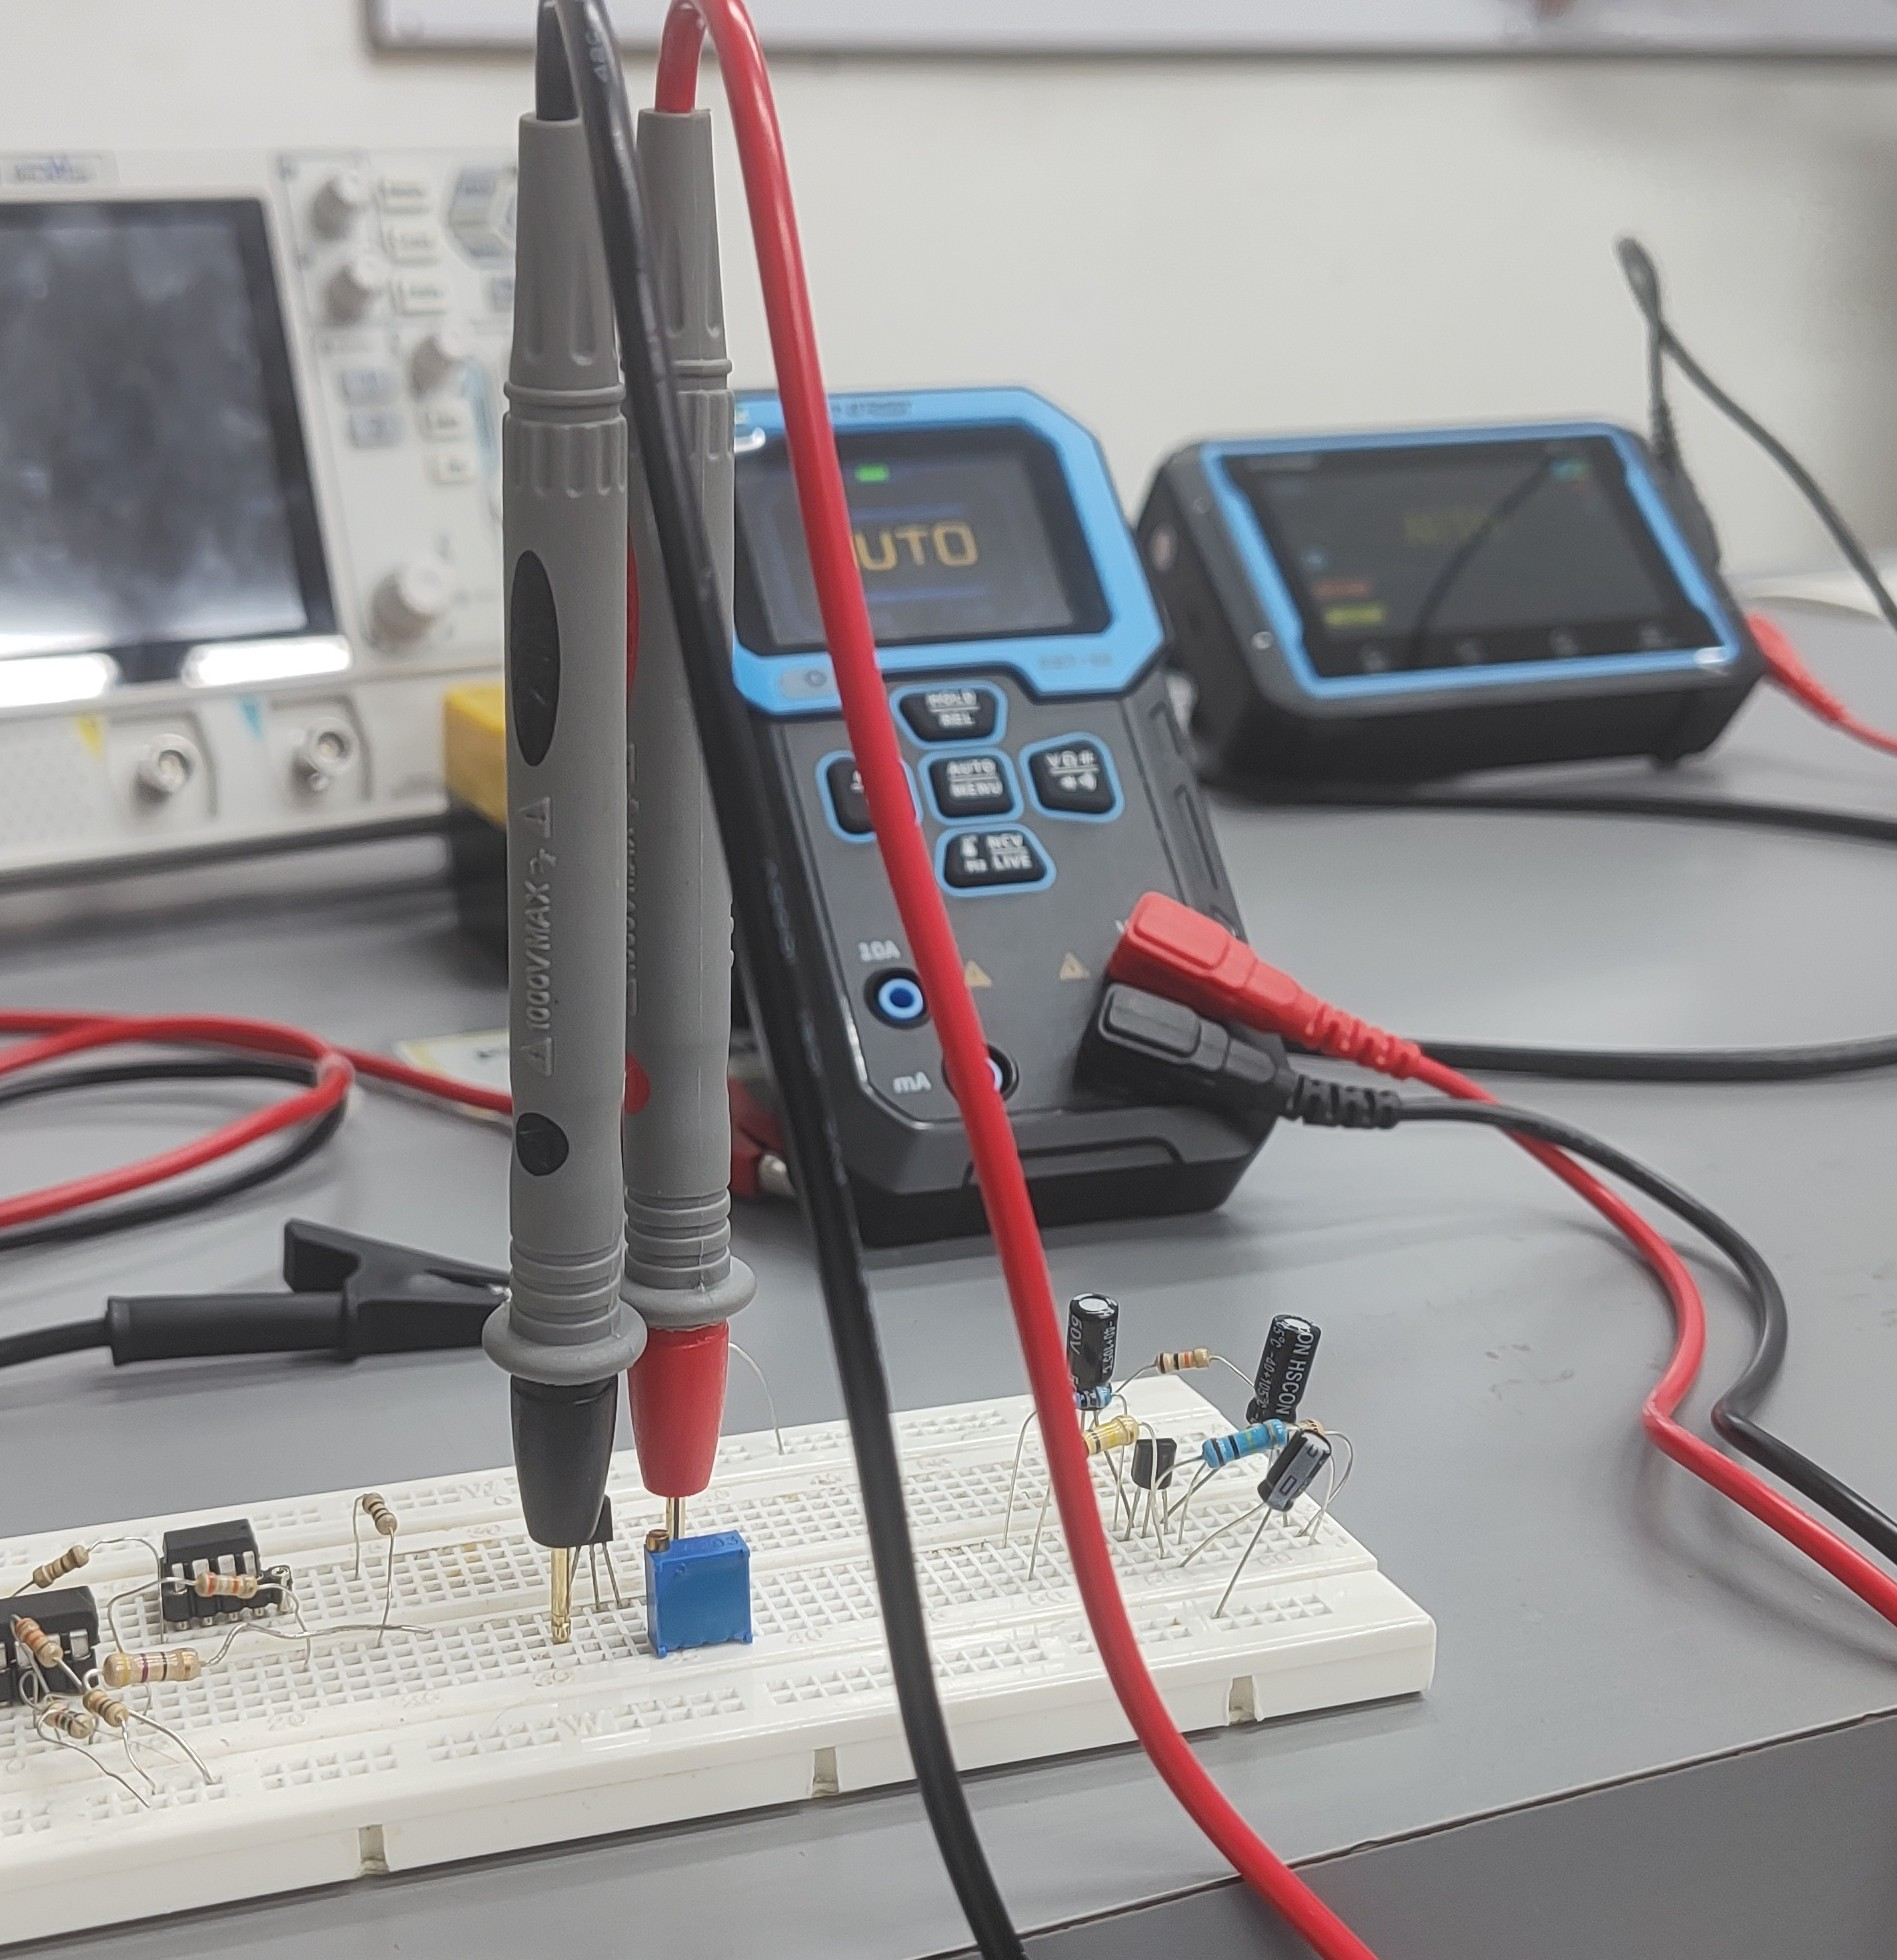
\includegraphics[width=\linewidth,height=0.95in,keepaspectratio]{caracterización_del_MOSFET.jpg}\\[1pt]
{\footnotesize (a)}
\end{minipage}\hfill
\begin{minipage}[t]{0.19\textwidth}
\centering
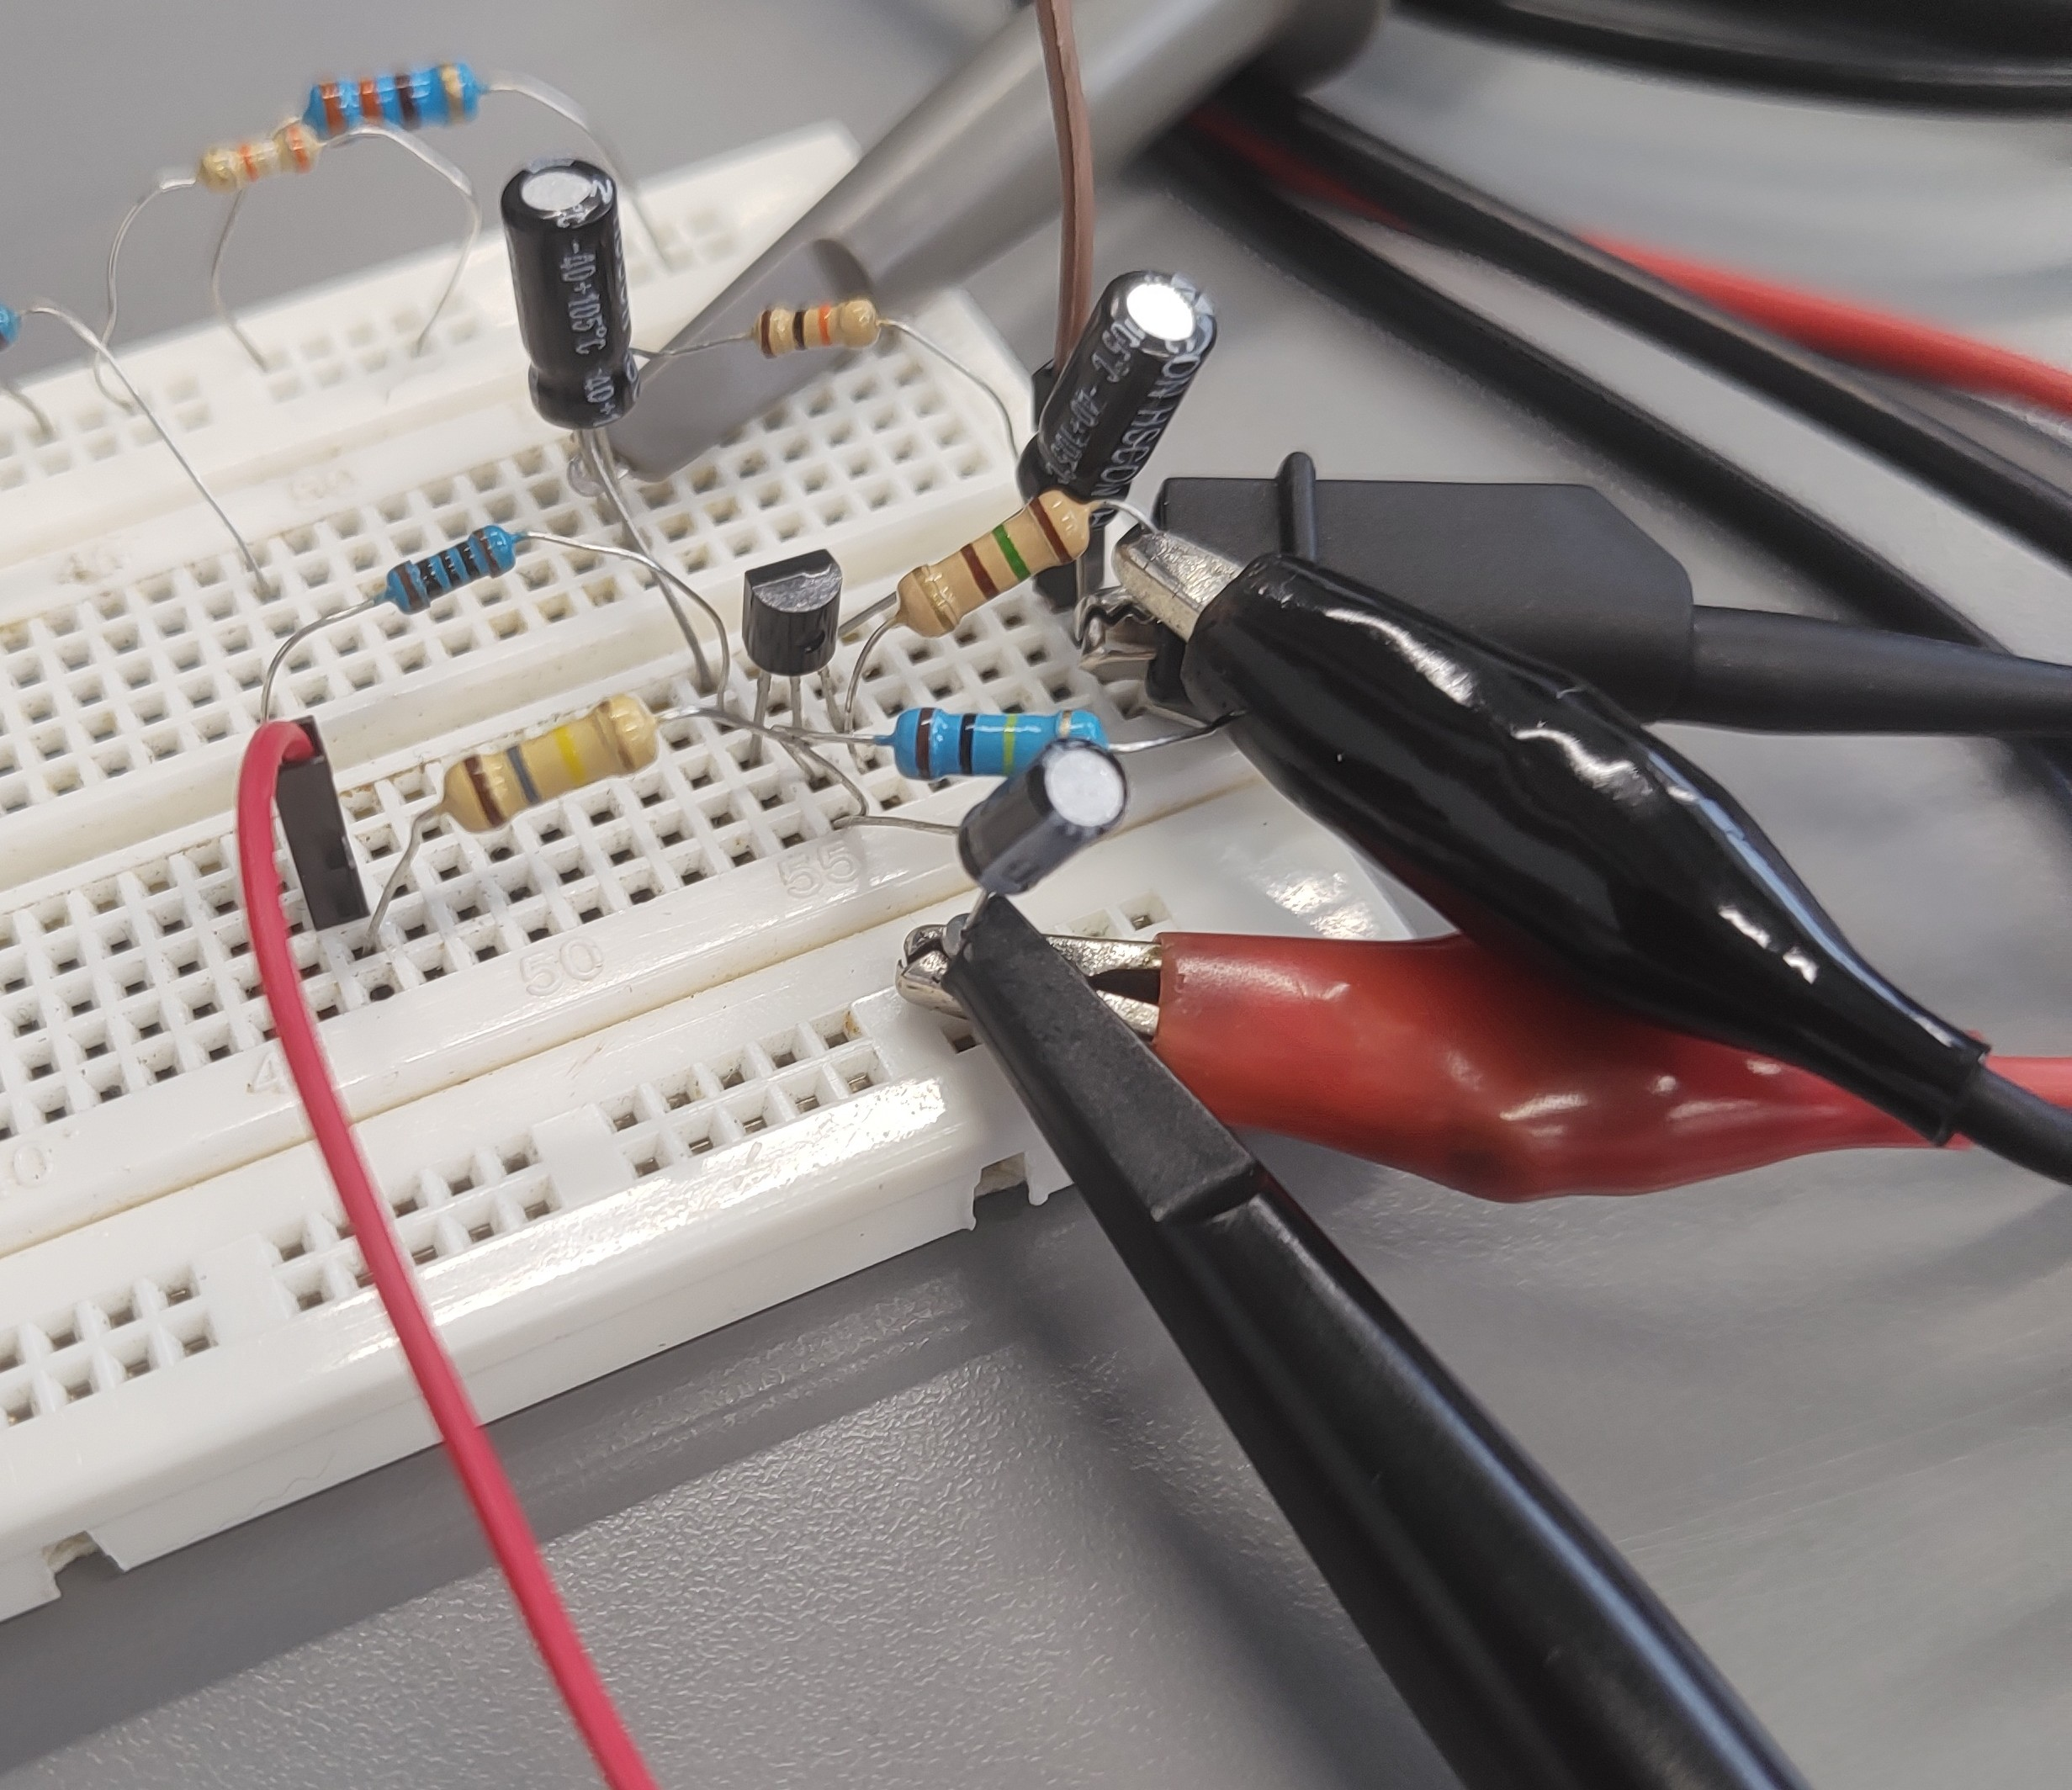
\includegraphics[width=\linewidth,height=0.95in,keepaspectratio]{Source_común.jpg}\\[1pt]
{\footnotesize (b)}
\end{minipage}\hfill
\begin{minipage}[t]{0.19\textwidth}
\centering
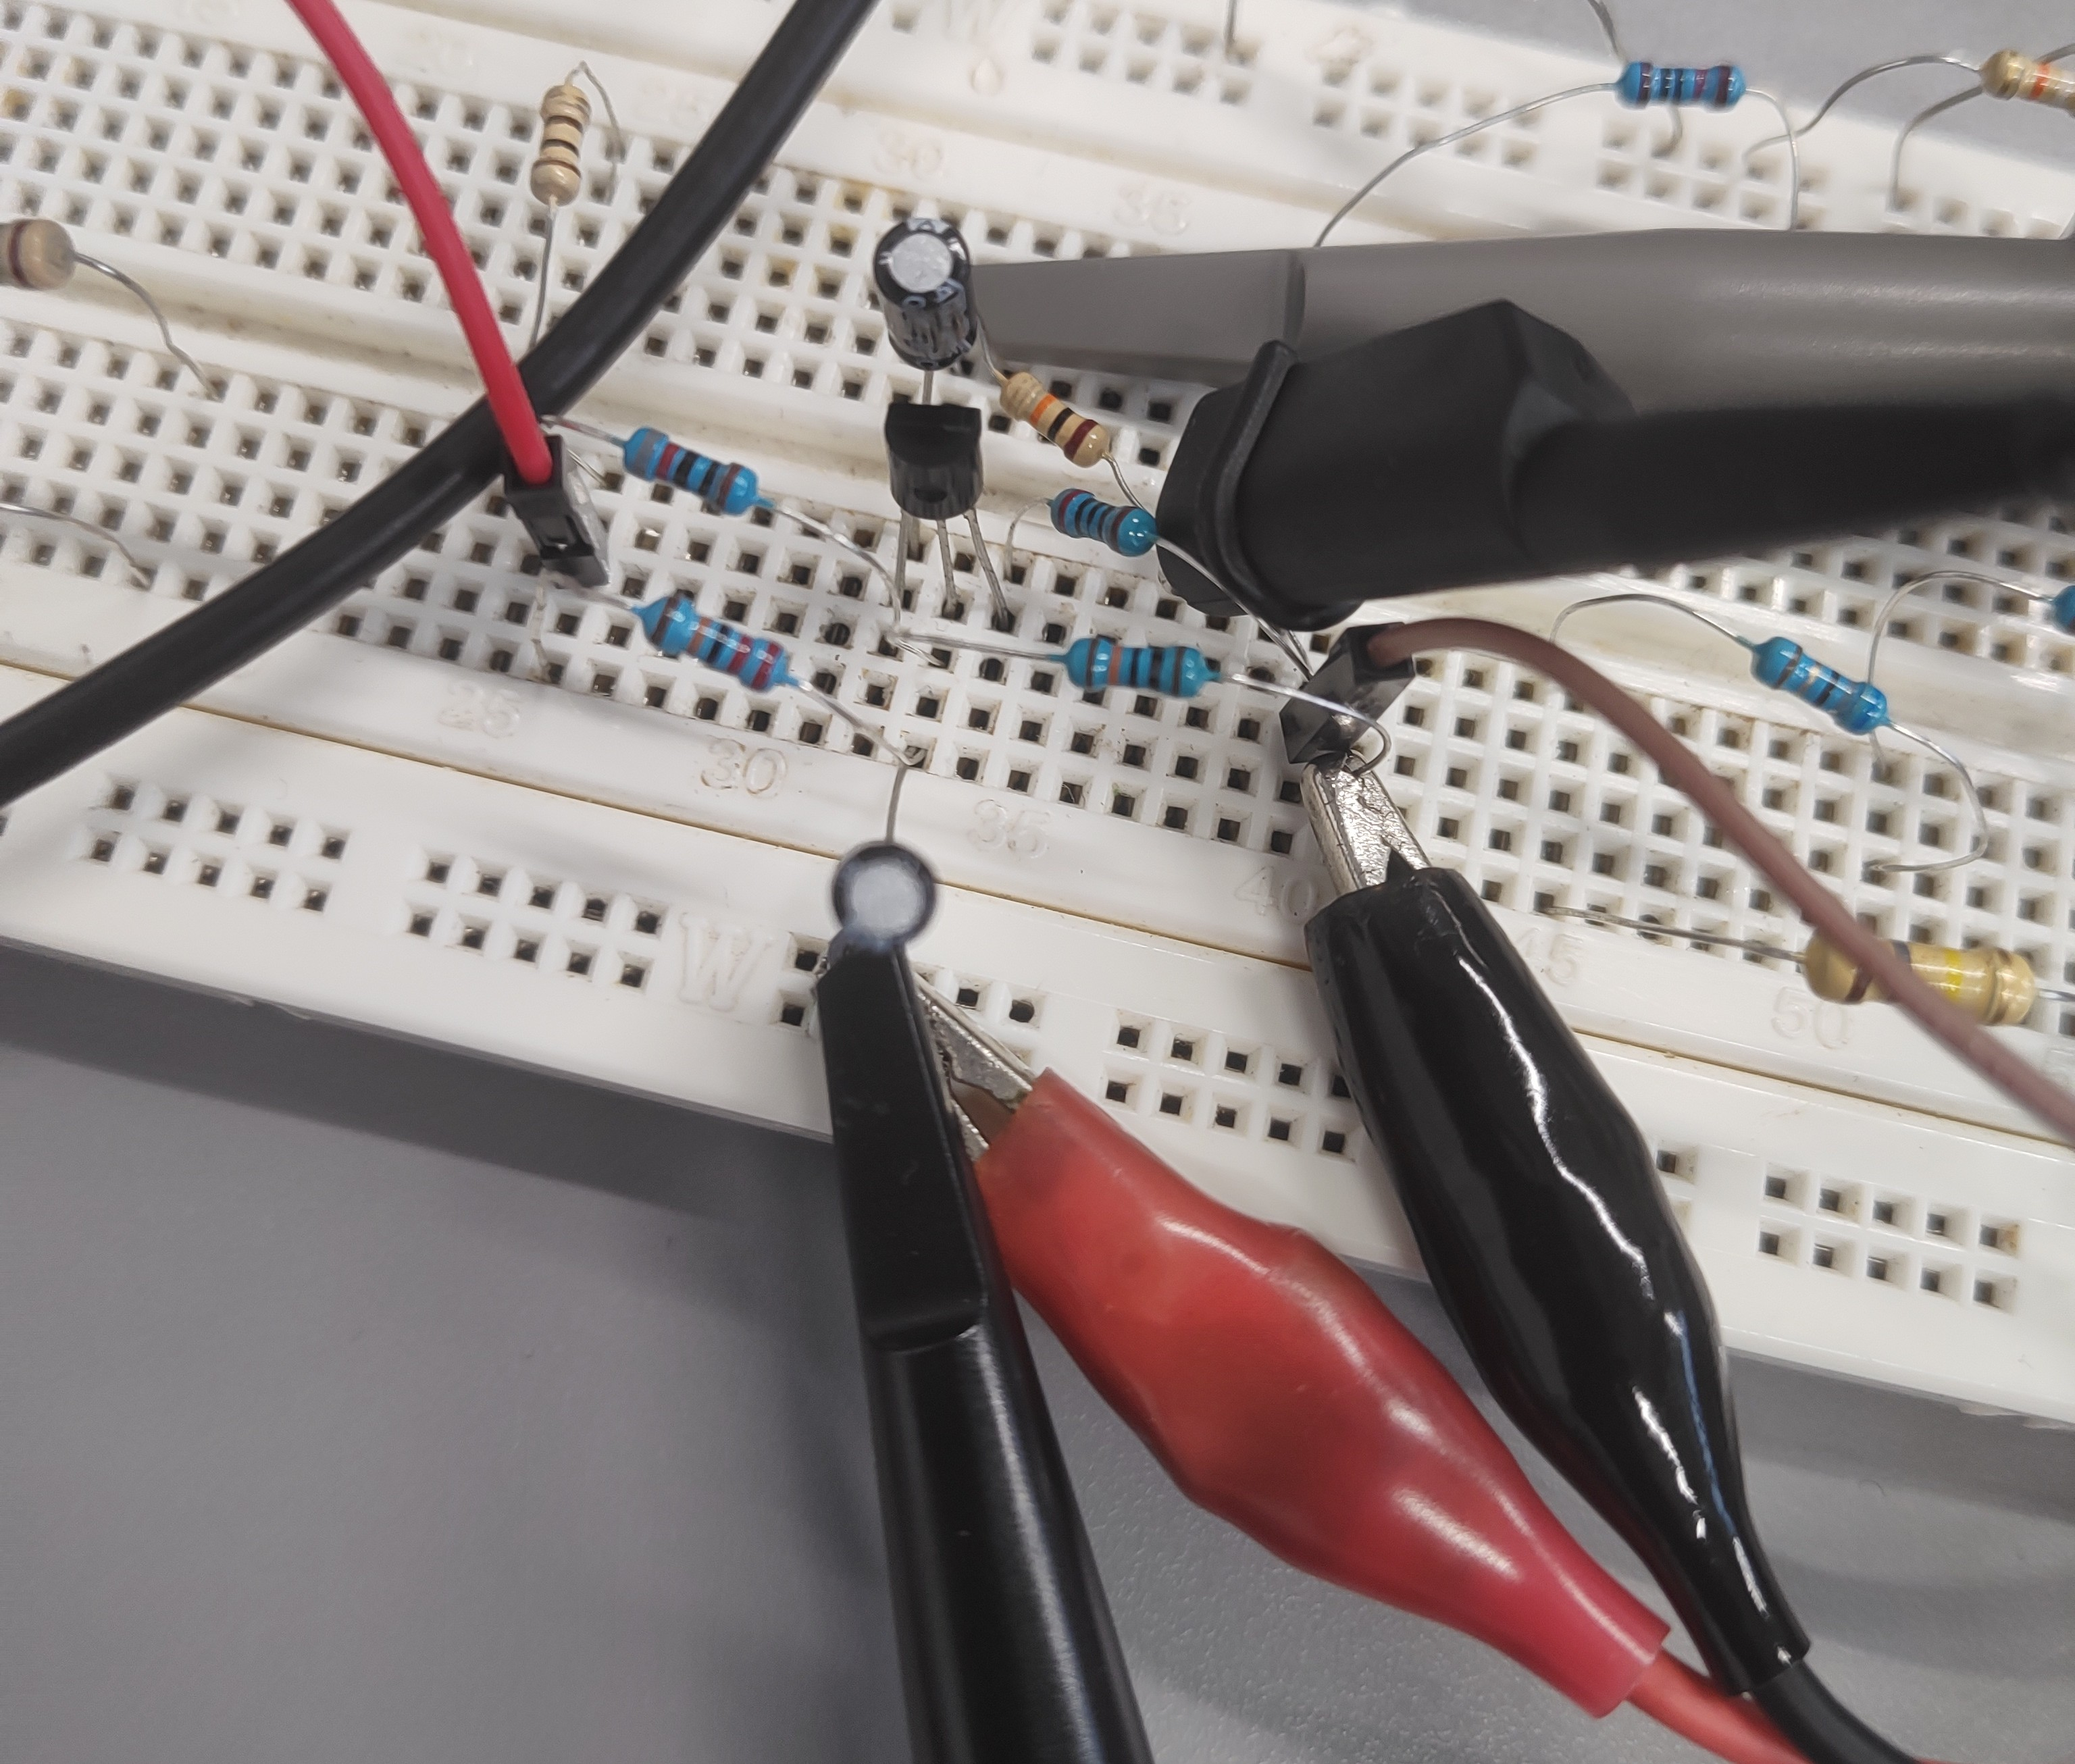
\includegraphics[width=\linewidth,height=0.95in,keepaspectratio]{source_degenerada.jpg}\\[1pt]
{\footnotesize (c)}
\end{minipage}\hfill
\begin{minipage}[t]{0.19\textwidth}
\centering
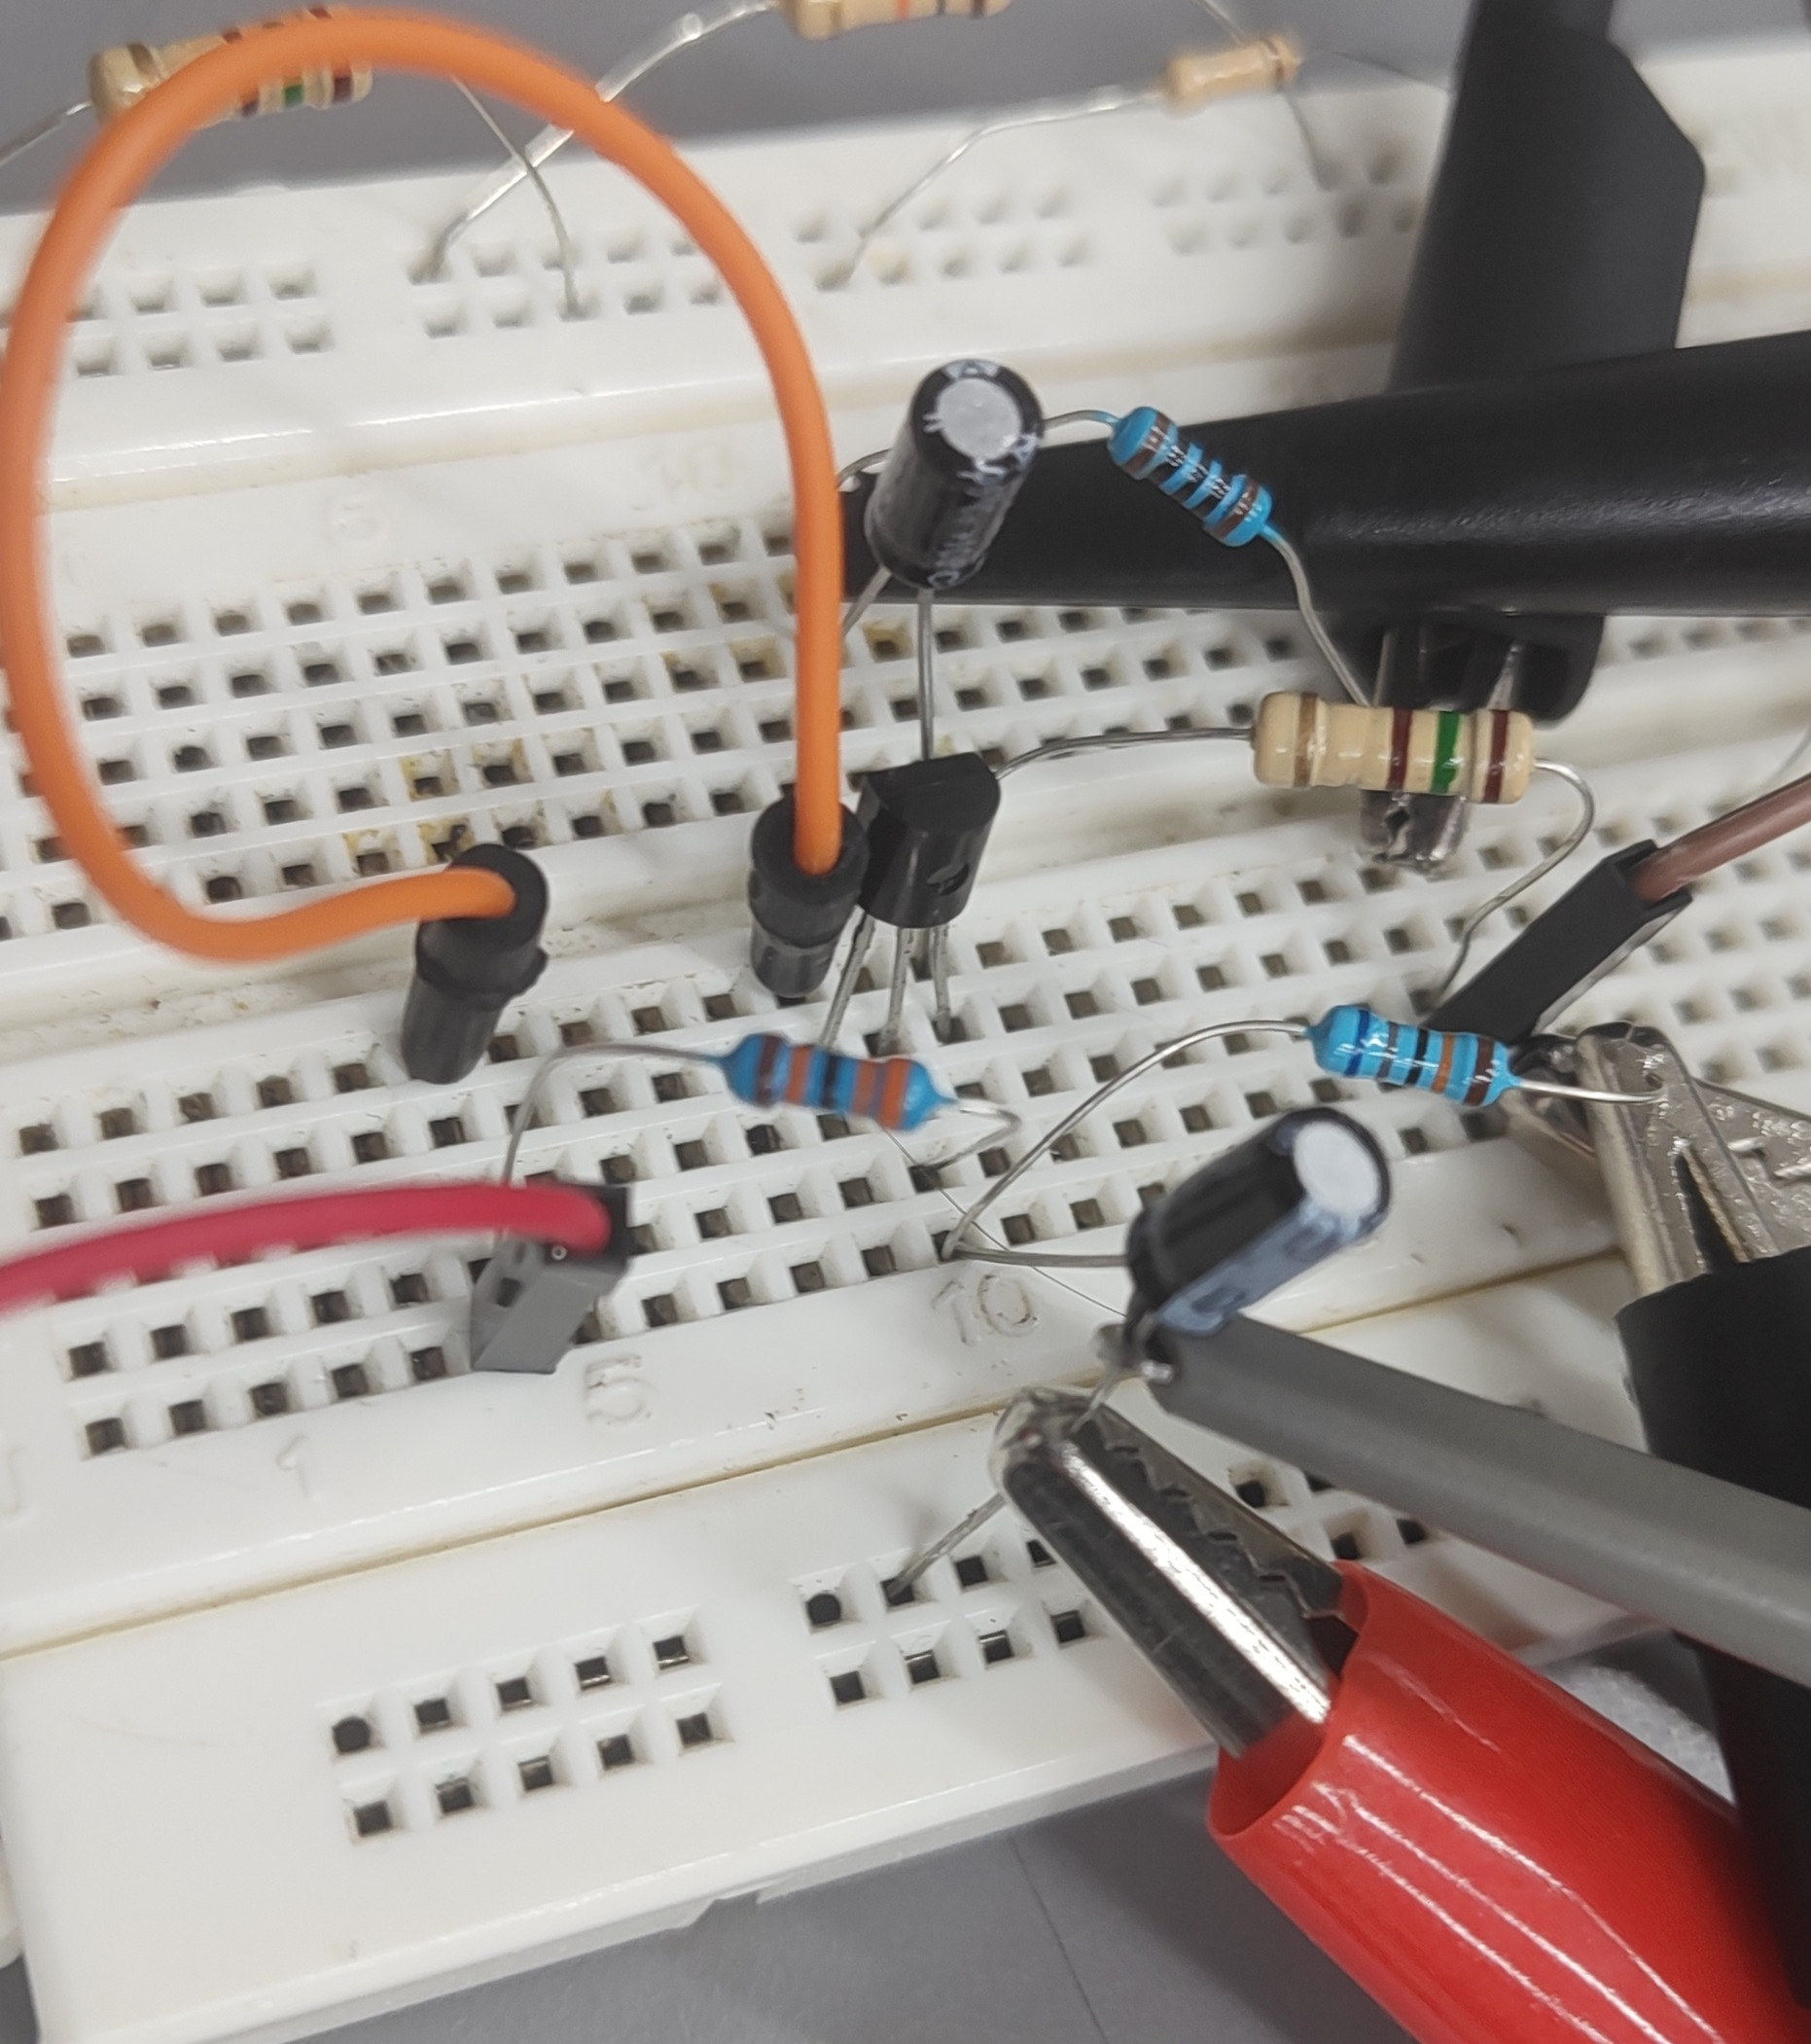
\includegraphics[width=\linewidth,height=0.95in,keepaspectratio]{drain_común.jpg}\\[1pt]
{\footnotesize (d)}
\end{minipage}\hfill
\begin{minipage}[t]{0.19\textwidth}
\centering
\includegraphics[width=\linewidth,height=0.95in,keepaspectratio]{cascada.jpg}\\[1pt]
{\footnotesize (e)}
\end{minipage}
\caption{Montajes experimentales: (a) caracterización del 2N7000 (Fig.~\ref{fig:circ_car}(a)); (b) amplificador de fuente común; (c) fuente degenerada; (d) drenador común; (e) cascada.}
\label{fig:montajes}
\end{figure*}

\subsection{Caracterización de dos ejemplares del 2N7000}
\label{sec:mont_car}
Con la topología de la Fig.~\ref{fig:circ_car}(a) se midieron $V_{GS}$ e $I_D$ de dos ejemplares del 2N7000 (Fig.~\ref{fig:montajes}(a)): un voltímetro en paralelo con $V_{GS}$ y un amperímetro en serie con el drenador. Se varió $R_1$ de 1 a \SI{10}{k\ohm} en pasos de \SI{1}{k\ohm} con un potenciómetro trimmer (Tabla~\ref{tab:car}). El ajuste por mínimos cuadrados de $\sqrt{I_D}$ contra $V_{GS}$ según la \eqref{eq:raiz} da, junto con la \eqref{eq:vt_kn},
\begin{equation}
\begin{aligned}
\text{Ejemplar 1: }&\sqrt{I_D}=0.1572\,V_{GS}-0.2208,\ R^2=0.9896,\\
\text{Ejemplar 2: }&\sqrt{I_D}=0.1486\,V_{GS}-0.2142,\ R^2=0.9738,
\end{aligned}
\label{eq:recta_m}
\end{equation}
de donde $\Vtm=\SI{1.405}{V}$ y $\knm=\SI{49.41}{mA/V^2}$ para el ejemplar 1, y $V_t=\SI{1.441}{V}$ y $\kn=\SI{44.18}{mA/V^2}$ para el ejemplar 2. Con el par de puntos $R_1=\SI{5}{k\ohm}$ la \eqref{eq:kn_punto} da $\kn=\SI{46.60}{mA/V^2}$ (ejemplar 1) y \SI{39.93}{mA/V^2} (ejemplar 2), que difieren \SI{5.68}{\percent} y \SI{9.62}{\percent} de los del ajuste.

\begin{table*}[htbp]
\centering
\caption{Caracterización con $R_1$ variable: mediciones de dos ejemplares del 2N7000 y simulación (Sec.~\ref{sec:sim_car}); error relativo de la simulación respecto al ejemplar 1 medido.}
\label{tab:car}
\scriptsize
\renewcommand{\arraystretch}{1.03}
\setlength{\tabcolsep}{5pt}
\begin{tabular}{@{}ccccccccc@{}}
\toprule
Condición & \multicolumn{2}{c}{Ejemplar 1 (med.)} & \multicolumn{2}{c}{Ejemplar 2 (med.)} & \multicolumn{2}{c}{Simulación} & \multicolumn{2}{c}{Error sim. vs. ej. 1} \\
\cmidrule(lr){2-3}\cmidrule(lr){4-5}\cmidrule(lr){6-7}\cmidrule(lr){8-9}
$R_1$ (k$\Omega$) & $V_{GS}$ (V) & $I_D$ (mA) & $V_{GS}$ (V) & $I_D$ (mA) & $V_{GS}$ (V) & $I_D$ (mA) & $V_{GS}$ (\%) & $I_D$ (\%) \\
\midrule
1 & 1.752 & 3.200 & 1.799 & 3.140 & 1.7816 & 3.2184 & 1.69 & 0.57 \\
2 & 1.669 & 1.636 & 1.720 & 1.641 & 1.7117 & 1.6442 & 2.56 & 0.50 \\
3 & 1.627 & 1.117 & 1.676 & 1.110 & 1.6765 & 1.1078 & 3.04 & 0.82 \\
4 & 1.594 & 0.808 & 1.647 & 0.840 & 1.6535 & 0.8366 & 3.73 & 3.54 \\
5 & 1.578 & 0.698 & 1.626 & 0.680 & 1.6366 & 0.6727 & 3.71 & 3.62 \\
6 & 1.559 & 0.569 & 1.609 & 0.572 & 1.6232 & 0.5628 & 4.12 & 1.09 \\
7 & 1.542 & 0.463 & 1.595 & 0.491 & 1.6123 & 0.4840 & 4.56 & 4.54 \\
8 & 1.534 & 0.434 & 1.582 & 0.429 & 1.6030 & 0.4246 & 4.50 & 2.17 \\
9 & 1.523 & 0.385 & 1.570 & 0.383 & 1.5950 & 0.3783 & 4.73 & 1.74 \\
10 & 1.515 & 0.349 & 1.541 & 0.347 & 1.5880 & 0.3412 & 4.82 & 2.23 \\
\bottomrule
\end{tabular}
\end{table*}

\subsection{Amplificadores de fuente común y fuente degenerada}
\label{sec:mont_fc}
Para el amplificador de fuente común se siguió la topología simulada (Fig.~\ref{fig:cs}; Fig.~\ref{fig:montajes}(b)). Para acercarse a $R_D=\SI{160}{\ohm}$ se usaron resistencias de \SI{100}{\ohm} y \SI{68}{\ohm} en serie (esta última, escasa); como la topología es muy sensible a los efectos termoeléctricos y a las tolerancias del semiconductor, para obtener la ganancia pedida se retiró después la de \SI{68}{\ohm}, dejando $R_D=\SI{100}{\ohm}$; los capacitores fueron electrolíticos. El amplificador de fuente degenerada (Fig.~\ref{fig:montajes}(c)) omite el capacitor en paralelo con $R_S$ y, gracias a la estabilidad de esta topología, no difiere del diseño.

Ambos se midieron con el osciloscopio Tektronix TBS1102B-EDU (acoplamiento AC, sonda 1X, \SI{50}{\micro s}/div, 2\,500 puntos exportados en CSV; salida en CH1 y entrada en CH2). Como el ruido de banda ancha infla el $V_{pp}$ que reporta el osciloscopio, las amplitudes se obtuvieron ajustando por mínimos cuadrados una sinusoide a cada registro, y el $HD_2$ con la proyección de Fourier sobre un número entero de periodos. Con la entrada en $\SI{98.8}{mV_{pp}}$ ($\hat v_{in}\approx\SI{50}{mV}$) la fuente común entregó $\SI{523.2}{mV_{pp}}$ y la degenerada $\SI{328.7}{mV_{pp}}$ con $\SI{98.6}{mV_{pp}}$ de entrada (Tabla~\ref{tab:med}, Fig.~\ref{fig:med}(a) y (b)); en ambos casos la salida está invertida.

\subsection{Amplificador de drenador común}
\label{sec:mont_dc}
El seguidor se montó con el mismo MOSFET de la fuente degenerada (Fig.~\ref{fig:montajes}(d)); su peculiaridad es que exigió resistencias de mayor potencia para manejar las corrientes. Se midió con el osciloscopio Rigol DHO812 (\SI{20}{\micro s}/div, \SI{31.25}{MSa/s}, 10\,000 puntos) con la entrada en C2 y la salida en C1, con $\SI{199.4}{mV_{pp}}$ de entrada y $\SI{179.9}{mV_{pp}}$ de salida (ajuste sinusoidal; Tabla~\ref{tab:med}, Fig.~\ref{fig:med}(c)), en fase con la entrada. La salida presenta picos de ruido de conmutación que elevan el $V_{pp}$ de pantalla (\SI{197.92}{mV} frente a \SI{201.88}{mV}).

\subsection{Amplificador en cascada}
\label{sec:mont_casc}
En esta configuración (Fig.~\ref{fig:montajes}(e)) se hicieron varios cambios respecto al diseño original: además de los ya mencionados respecto a la fuente común, ambas etapas se alimentaron con una fuente lineal de \SI{12}{V} en lugar de la conmutada del laboratorio. Como el circuito no pudo presentarse durante las horas de clase, se presentó en un horario sin préstamo de equipos, por lo que se empleó otra instrumentación: Un osciloscopio portátil FNIRSI 2C53P de dos canales, y el generador de ondas de un FNIRSI DSO-153 (sinusoide de \SI{10}{kHz} y \SI{0.1}{V_{pp}}). El ajuste del osciloscopio se encuentra a:  \SI{100}{mV}/div, con CH1 (entrada) en acoplamiento AC y CH2 (salida) en DC. Con $\SI{34.37}{mV_{rms}}$ de entrada la salida fue de $\SI{165.62}{mV_{rms}}$ (Fig.~\ref{fig:med}(d), en contrafase; Tabla~\ref{tab:med}); el $V_{pp}$ de la salida, \SI{506.25}{mV}, supera $2\sqrt2$ veces su valor eficaz, lo que indica picos o distorsión.

\begin{table}[htbp]
\centering
\caption{Resultados medidos a 10 kHz de los amplificadores de fuente común (FC), fuente degenerada (FD), drenador común (DC) y cascada.}
\label{tab:med}
\scriptsize
\renewcommand{\arraystretch}{1.03}
\setlength{\tabcolsep}{3pt}
\begin{tabular}{@{}lcccc@{}}
\toprule
Magnitud & FC & FD & DC & Cascada \\
\midrule
$v_{in,rms}$ (mV) & 35.0 & 35.0 & 70.5 & 34.37 \\
$v_{out,rms}$ (mV) & 185.2 & 116.4 & 63.6 & 165.62 \\
$|A_v|$, razón de valores eficaces (V/V) & 5.29 & 3.33 & 0.902 & 4.82 \\
$|A_v|$, razón de $V_{pp}$ de pantalla (V/V) & 4.98 & 3.16 & 0.980 & 5.23 \\
$\angle A_v$ & $164.7^\circ$ & $-159.2^\circ$ & $1.7^\circ$ & contrafase \\
$HD_2$ (\%) & 3.67 & $\le0.12$ & --- & --- \\
\bottomrule
\end{tabular}
\end{table}

\begin{figure*}[htbp]
\centering
% USUARIO: fig_med_fc.pdf, fig_med_fd.pdf y fig_med_dc.pdf se generan con graficar_mediciones.py a partir de los CSV;
% cascada_toma_de_datos.jpg es la captura de pantalla del osciloscopio portátil.
\begin{minipage}[b]{0.238\textwidth}
\centering
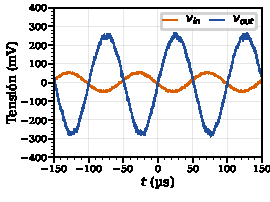
\includegraphics[width=\linewidth]{fig_med_fc.pdf}\\[1pt]
{\footnotesize (a)}
\end{minipage}\hfill
\begin{minipage}[b]{0.238\textwidth}
\centering
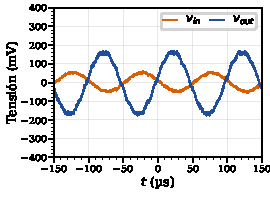
\includegraphics[width=\linewidth]{fig_med_fd.pdf}\\[1pt]
{\footnotesize (b)}
\end{minipage}\hfill
\begin{minipage}[b]{0.238\textwidth}
\centering
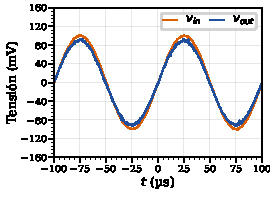
\includegraphics[width=\linewidth]{fig_med_dc.pdf}\\[1pt]
{\footnotesize (c)}
\end{minipage}\hfill
\begin{minipage}[b]{0.268\textwidth}
\centering
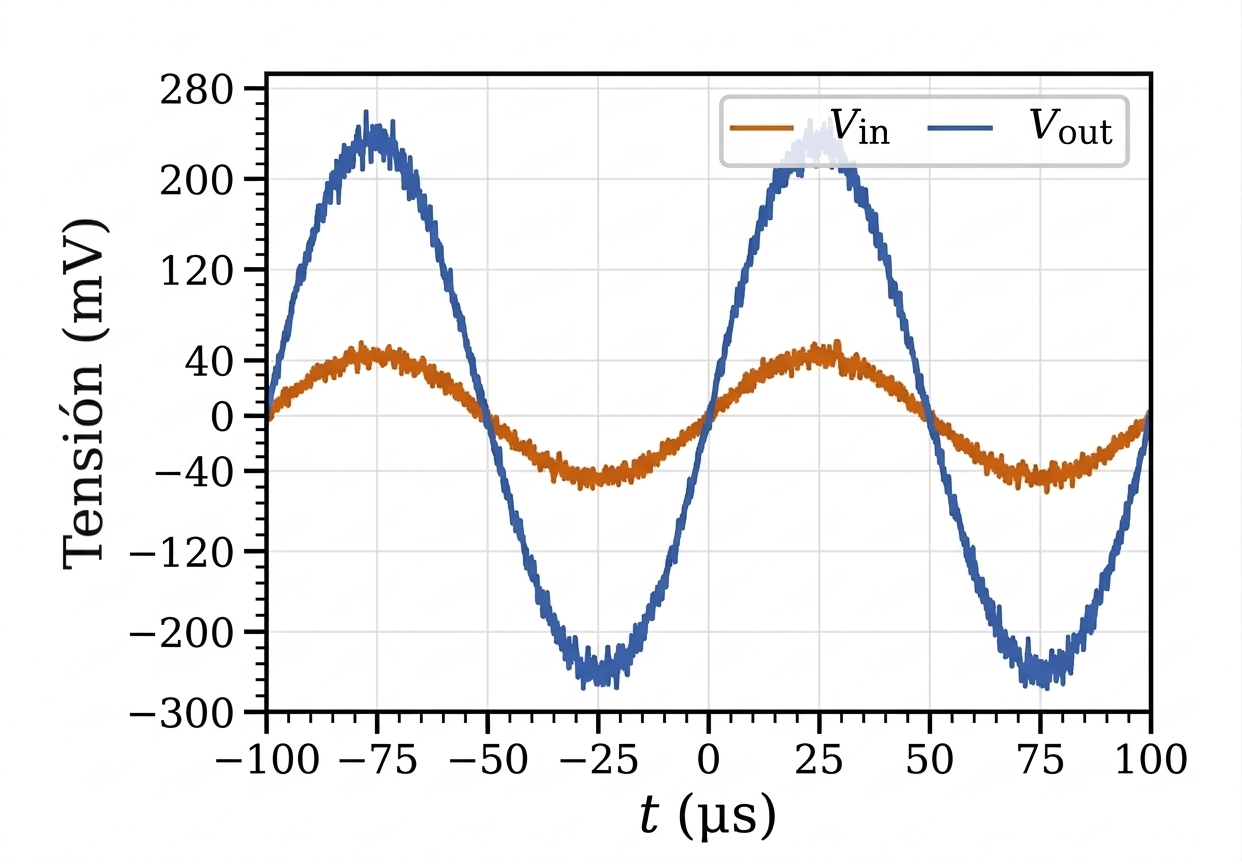
\includegraphics[width=\linewidth]{cascada_toma_de_datos.jpg}\\[1pt]
{\footnotesize (d)}
\end{minipage}
\caption{Señales de entrada y salida medidas a 10 kHz: (a) fuente común; (b) fuente degenerada (TBS1102B-EDU, $v_{in}$ en CH2 y $v_{out}$ en CH1); (c) drenador común (DHO812, $v_{in}$ en C2 y $v_{out}$ en C1); (d) cascada (captura de pantalla; CH1 entrada y CH2 salida).}
\label{fig:med}
\end{figure*}

%==================================================================
\section{Análisis de resultados}
%==================================================================

\subsection{Caracterización del MOSFET}
En la Fig.~\ref{fig:car_sim}(a) $\sqrt{I_D}$ crece linealmente con $V_{GS}$ ($R^2=0.9932$) porque en saturación la \eqref{eq:sat} implica $\sqrt{I_D}\propto V_{GS}-V_t$ (\eqref{eq:raiz}); el intercepto es $V_t$ porque allí $\sqrt{I_D}=0$, es decir, $V_{GS}=V_t$. El transistor de la Fig.~\ref{fig:circ_car}(a) está en saturación, pues $V_{DS}=V_{GS}>V_{GS}-V_t$, y permanece allí para cualquier $R_1$ porque este solo desplaza el punto según la \eqref{eq:kvl_car} sin romper esa igualdad \cite{sedra}. $\Vts=\SI{1.496}{V}$ está dentro del rango de la hoja de datos y el $\kn$ puntual difiere \SI{4.59}{\percent} del de la pendiente; las mediciones (\eqref{eq:recta_m}) siguen la misma tendencia, con interceptos de \SI{1.405}{V} y \SI{1.441}{V}.

La Tabla~\ref{tab:car} compara el ejemplar 1 con la simulación: las corrientes difieren en promedio \SI{2.08}{\percent} (máximo \SI{4.54}{\percent}) y las tensiones $V_{GS}$ \SI{3.75}{\percent} (máximo \SI{4.82}{\percent}), pero $\Vts$ es \SI{6.48}{\percent} mayor que $\Vtm$ y $\kns=\SI{71.52}{mA/V^2}$ es \SI{44.76}{\percent} mayor que $\knm$: el modelo de LTspice reproduce $I_D$ y $V_{GS}$ en el punto de medida, pero no los parámetros. Entre los dos ejemplares, $V_t$ difiere \SI{2.60}{\percent} y $\kn$ \SI{10.57}{\percent}, por lo que los parámetros deben medirse en cada ejemplar y compararse al elegir el par del espejo.

\subsection{Curvas características y parámetros de operación}
\label{sec:an_curvas}
La Fig.~\ref{fig:car_sim}(b) permite identificar las regiones de operación: la corriente de saturación crece con $V_{GS}$ y es casi independiente de $V_{DS}$ tras la frontera de la \eqref{eq:frontera}. Estas familias de curvas son importantes porque muestran gráficamente esa frontera y permiten fijar un punto de polarización donde la oscilación de la señal no empuje al transistor a triodo; y son específicas del dispositivo caracterizado porque dependen de su $V_t$ y $\kn$, que varían entre ejemplares de la misma referencia (\SI{2.60}{\percent} y \SI{10.57}{\percent} en los dos medidos). La \eqref{eq:sat} con la \eqref{eq:param_op} reproduce las corrientes simuladas con errores de \SI{1.84}{\percent}, \SI{1.70}{\percent} y \SI{0.56}{\percent} para $V_{GS}$ de 2, 2.5 y 3 V, y de \SI{4.09}{\percent} y \SI{8.04}{\percent} para 3.5 y 4 V, mientras que con los parámetros de la \eqref{eq:recta}, obtenidos cerca del umbral, subestima la corriente entre \SI{30.5}{\percent} y \SI{43.1}{\percent}, porque la pendiente de $\sqrt{I_D}$ crece con $V_{GS}$ (de \SI{0.19}{A^{1/2}/V} a \SI{0.26}{A^{1/2}/V}). Por eso $V_t$ y $\kn$ deben extraerse cerca de la zona de operación, lo que afecta a los parámetros medidos ($V_{GS}\le\SI{1.752}{V}$) pues los amplificadores operan con $V_{GS}\approx\SI{2.05}{V}$. Para $V_{GS}\ge\SI{3.5}{V}$ la corriente supera los \SI{200}{mA} y la potencia \SI{1}{W}, por lo que el barrido de laboratorio debe restringirse.

\subsection{Diseño de los amplificadores}
\label{sec:an_dis}
Para garantizar amplificación se requiere saturación ($V_{DS}\ge\Vov$), una $\gm$ adecuada, capacitores que sean cortocircuitos a la frecuencia de trabajo (\eqref{eq:fc}), señales dentro del límite de pequeña señal ($v_{gs}\ll2\Vov$) y corriente y potencia dentro de la Tabla~\ref{tab:datasheet} \cite{sedra,datasheet}. La Tabla~\ref{tab:param} muestra que los tres amplificadores cumplen la saturación y consumen menos de \SI{1}{W}. En la fuente común $|A_v|=4.99$ se desvía \SI{0.2}{\percent} de 5; en la degenerada $|A_v|=3.38$ supera en \SI{12.7}{\percent} el valor de 3 y la salida de \SI{338}{mV_{pp}} cumple el mínimo de 300 mV$_{pp}$. El drenador común tiene ganancia menor que 1 y la menor $Z_{out}$ (\eqref{eq:zout_cd}), a costa de una corriente cinco veces mayor. El drenador común y el espejo se calcularon con parámetros extraídos con $I_D\le\SI{3.2}{mA}$, por lo que su corriente real, en efecto podía ser mayor (Sec.~\ref{sec:an_curvas}).

\subsection{Fuentes común y degenerada: teoría frente a simulación}
\label{sec:an_amp}
\textit{Fuente común.} Según la Fig.~\ref{fig:transf} y la Tabla~\ref{tab:sim}, la simulación es lineal para entradas pequeñas y se comprime al crecer la amplitud: $|A_v|$ cae \SI{0.46}{\percent} con 50 mV y \SI{7.61}{\percent} con 200 mV. El $HD_2$ se duplica al duplicar la amplitud de 10 a 20 mV, como predice la \eqref{eq:hd2}, y cruza el \SI{5}{\percent} en $\hat v_{in}\approx\SI{72}{mV}$ (con 50 mV es \SI{3.45}{\percent}). Con $\Vtm$ y $\knm$ la ganancia calculada queda \SI{43.1}{\percent} por debajo de la simulada (4.99 frente a 8.77; Tabla~\ref{tab:cmp}), por lo que en simulación no se cumple $|v_{out}|\approx5|v_{in}|$. La causa es la extrapolación de la Sec.~\ref{sec:an_curvas}: con $\Vtp$ y $\knp$ la \eqref{eq:vov} da $\Vov=\SI{0.395}{V}$, $I_D=\SI{10.77}{mA}$ y $\gm=\SI{54.54}{mS}$, de modo que $I_D$ aumenta solo \SI{5.9}{\percent} (la autopolarización con $R_S$ lo fija casi sin importar $\kn$) pero $\gm=\sqrt{2\kn I_D}$ aumenta \SI{72}{\percent}; con ello la \eqref{eq:Av} da $-8.59$ y las desviaciones frente a la simulación son de solo \SI{2.1}{\percent} en $A_v$, \SI{8.2}{\percent} en $HD_2$ y \SI{9.6}{\percent} en el límite de pequeña señal. En el montaje cabe esperar $|A_v|>4.99$ y un límite menor que \SI{128}{mV}.

\begin{table}[htbp]
\centering
\caption{Simulación frente a teoría con parámetros medidos ($\Vtm$, $\knm$) y del modelo en la zona de operación ($\Vtp$, $\knp$), con $\hat v_{in}=\SI{50}{mV}$. Errores respecto a la simulación; $\gm$ equivalente despejado de la \eqref{eq:Av_deg}.}
\label{tab:cmp}
\scriptsize
\renewcommand{\arraystretch}{1.03}
\setlength{\tabcolsep}{2.5pt}
\begin{tabular}{@{}lccccc@{}}
\toprule
Magnitud & Sim. & $\Vtm,\knm$ & Error (\%) & $\Vtp,\knp$ & Error (\%) \\
\midrule
\multicolumn{6}{@{}l}{\textit{Fuente común}} \\
$|A_v|$ (V/V) & 8.77 & 4.99 & \SI{43.1}{\percent} & 8.59 & \SI{2.1}{\percent} \\
$HD_2$ (\%) & 3.45 & 1.95 & \SI{43.4}{\percent} & 3.17 & \SI{8.2}{\percent} \\
$\hat v_{in,max}$, $HD_2\le\SI{5}{\percent}$ (mV) & 72 & 128 & \SI{77.9}{\percent} & 79 & \SI{9.6}{\percent} \\
\midrule
\multicolumn{6}{@{}l}{\textit{Fuente degenerada}} \\
$|A_v|$ (V/V) & 3.087 & 3.149 & \SI{2.0}{\percent} & 3.384 & \SI{9.6}{\percent} \\
$\gm$ equivalente (mS) & 21.98 & 24.58 & \SI{11.8}{\percent} & 41.75 & \SI{89.9}{\percent} \\
$HD_2$ (\%) & 0.0805 & 0.0718 & \SI{10.8}{\percent} & 0.0473 & \SI{41.2}{\percent} \\
\bottomrule
\end{tabular}
\end{table}

\textit{Fuente degenerada.} La característica es prácticamente lineal en todo el barrido: $|A_v|$ solo cae \SI{0.15}{\percent} entre 10 y 400 mV, la salida de \SI{308.5}{mV_{pp}} cumple el mínimo de 300 mV$_{pp}$ (margen de \SI{2.8}{\percent}) y el $HD_2$ de \SI{0.0805}{\percent} con 50 mV es unas 43 veces menor que el de la fuente común; con 400 mV no se alcanza el \SI{5}{\percent} porque $\hat v_{gs}=400/9.35=\SI{42.8}{mV}<0.2\,\Vov=\SI{60.5}{mV}$, de acuerdo con la \eqref{eq:limite_deg}. Con $\Vtp$ y $\knp$ la ganancia calculada difiere \SI{9.6}{\percent} de la simulada y el $\gm$ equivalente, \SI{21.98}{mS}, queda lejos de los \SI{41.75}{mS} calculados (\SI{89.9}{\percent}): es la misma extrapolación, pues esos parámetros se extrajeron con $I_D$ de decenas de mA y el amplificador opera con $I_D\approx\SI{6.3}{mA}$. Con los parámetros del ejemplar 1 los errores bajan a \SI{2.0}{\percent}, \SI{11.8}{\percent} y \SI{10.8}{\percent} (Tabla~\ref{tab:cmp}). La degeneración reduce la sensibilidad a los parámetros (error en $A_v$ de \SI{43.1}{\percent} a \SI{9.6}{\percent}) pero no elimina el error sistemático; conviene extraer $V_t$ y $\kn$ cerca de $I_D\approx\SI{6}{mA}$.

\subsection{Punto de operación, impedancias y drenador común}
\label{sec:an_op_zin}
El punto de operación simulado de la fuente común coincide con la teoría con un error máximo de \SI{0.51}{\percent} en $I_D$ y \SI{0.22}{\percent} en $V_{DS}$ (Tabla~\ref{tab:op}), lo que valida el diseño con los parámetros del ejemplar 1; en la degenerada el acuerdo es menor ($I_D$ \SI{8.3}{\percent}, $V_{DS}$ \SI{15.1}{\percent}) por la extrapolación hasta $I_D\approx\SI{6}{mA}$. Las impedancias simuladas a 10 kHz coinciden con las teóricas (\SI{0.0}{\percent}), lo que valida el modelo de pequeña señal y que a esa frecuencia los capacitores son cortocircuitos; $Z_{in}$ es alta (\SI{64}{k\ohm} y \SI{69}{k\ohm}, fijada por el divisor) y $Z_{out}=R_D$ es mayor en la degenerada (\SI{820}{\ohm} frente a \SI{160}{\ohm}) porque necesita un $R_D$ mayor para alcanzar su ganancia (\eqref{eq:Av_deg}).

En el drenador común (Sec.~\ref{sec:sim_cd}) la ganancia y el punto de operación coinciden con la teoría; la discrepancia en $Z_{out}$ (\SI{11.3}{\percent}) se debe a que la \eqref{eq:zout_cd} desprecia $r_o$ y las capacitancias parásitas, y el $HD_2$ simulado (\SI{0.0856}{\percent}) es muy bajo porque $v_{gs}\approx0.2\,v_{in}$, aunque supera en \SI{25.2}{\percent} al de la \eqref{eq:hd2_deg}, una aproximación a segundo orden.

\subsection{Respuesta en frecuencia y ancho de banda}
\label{sec:an_bode}
En la fuente común (Fig.~\ref{fig:bode}(a)) el corte inferior de $\approx\SI{310}{Hz}$ está dominado por $C_S$, cuyo polo teórico es $f_p=\SI{611}{Hz}$ (\eqref{eq:fc}; error de \SI{49.3}{\percent}); no hay corte superior hasta \SI{100}{MHz}, pues la baja resistencia vista por las capacitancias parásitas ($\approx\SI{157}{\ohm}$) desplaza ese polo por encima del barrido, y el ancho de banda es mayor que \SI{100}{MHz} (cota inferior). En la degenerada (Fig.~\ref{fig:bode}(b)) $f_L\approx\SI{465}{Hz}$ y $f_H\approx\SI{34}{MHz}$ dan un ancho de banda del orden de \SI{34}{MHz}; la muesca de \SI{63.4}{Hz} no corresponde a ningún polo o cero del diseño y puede deberse a la interacción de $C_1$ con la red de polarización o a la configuración del \texttt{.ac}, sin afectar la banda media. Los plateaus de \SI{5.66}{dB} y \SI{22.74}{dB} no coinciden con las ganancias transitorias (\SI{18.9}{dB} y \SI{9.8}{dB}) y en la FC la ganancia crece hacia baja frecuencia, contrario a lo esperado con $C_S$; por ello de estos barridos solo se toman las frecuencias de corte y la banda media se toma de los transitorios. El drenador común (Fig.~\ref{fig:cd}(b)) tiene teóricamente el menor corte inferior ($\approx\SI{140}{Hz}$, por $C_2$) y respuesta plana en $-1.92$ dB (curva teórica, sin barrido simulado). En la cascada (Fig.~\ref{fig:casc}(b)) la ganancia en banda media de \SI{4.42}{V/V} difiere \SI{4.1}{\percent} de los \SI{4.61}{V/V} de la \eqref{eq:Av_casc}, y $f_L\approx\SI{694}{Hz}$ y $f_H\approx\SI{15.1}{MHz}$ resultan peores que los de cada etapa, como es propio de una cascada. Así, el corte inferior crece de $\approx\SI{140}{Hz}$ (DC) a \SI{310}{Hz} (FC), \SI{465}{Hz} (FD) y \SI{694}{Hz} (cascada), y el ancho de banda baja de más de \SI{100}{MHz} (FC) a \SI{34}{MHz} (FD) y \SI{15.1}{MHz} (cascada).

\subsection{Resultados experimentales frente a teoría y simulación}
\label{sec:an_med}
Para comparar una medición $X_{med}$ con una referencia $X_{ref}$ (teórica o simulada) se reportan el error absoluto $|X_{med}-X_{ref}|$ y el error relativo porcentual
\begin{equation}
\varepsilon=\frac{|X_{med}-X_{ref}|}{|X_{ref}|}\times\SI{100}{\percent}.
\label{eq:err}
\end{equation}
La Tabla~\ref{tab:med_cmp} lo aplica a las ganancias de la Tabla~\ref{tab:med} frente a las de la Tabla~\ref{tab:param} y a las simulaciones de las Secs.~\ref{sec:sim_amp}, \ref{sec:sim_cd} y \ref{sec:sim_casc}.

\begin{table*}[htbp]
\centering
\caption{Medición frente a teoría y simulación (error absoluto y relativo, \eqref{eq:err}). Teoría: FC con $\Vtm,\knm$, FD con $\Vtp,\knp$.}
\label{tab:med_cmp}
\scriptsize
\renewcommand{\arraystretch}{1.03}
\setlength{\tabcolsep}{5pt}
\begin{tabular}{@{}llcccccccc@{}}
\toprule
Circuito & Magnitud & Medido & Teoría & Error abs. & Error (\%) & Simulación & Error abs. & Error (\%) \\
\midrule
FC & $|A_v|$ (V/V) & 5.29 & 4.99 & 0.30 & 6.1 & 8.77 & 3.48 & 39.6 \\
FC & $HD_2$ (\%) & 3.67 & 1.95 & 1.72 & 88.2 & 3.45 & 0.22 & 6.4 \\
FD & $|A_v|$ (V/V) & 3.33 & 3.38 & 0.05 & 1.5 & 3.087 & 0.245 & 7.9 \\
DC & $|A_v|$ (V/V) & 0.902 & 0.801 & 0.101 & 12.6 & 0.8013 & 0.101 & 12.6 \\
Cascada & $|A_v|$ (V/V) & 4.82 & 4.61 & 0.21 & 4.5 & 4.58 & 0.24 & 5.2 \\
\bottomrule
\end{tabular}
\end{table*}

\textit{Fuente común.} La ganancia medida (5.29) cumple el objetivo de 5 con \SI{6.1}{\percent} de error, pero difiere \SI{39.6}{\percent} de la simulada (8.77) porque el montaje usó $R_D=\SI{100}{\ohm}$ y no los \SI{160}{\ohm} simulados. Con $R_D\parallel R_L=\SI{99.0}{\ohm}$ y la \eqref{eq:Av}, la ganancia medida implica $\gm\approx\SI{53.5}{mS}$, que difiere \SI{2.0}{\percent} de los \SI{54.54}{mS} del modelo con $\Vtp,\knp$ (con ese $\gm$ la \eqref{eq:Av} da 5.40) y está muy lejos de los \SI{31.69}{mS} con $\Vtm,\knm$ (que darían 3.14): la medición confirma lo previsto en la Sec.~\ref{sec:an_amp}, pues los parámetros extraídos cerca del umbral subestiman $\gm$. El $HD_2$ medido con $\hat v_{in}\approx\SI{49}{mV}$, \SI{3.67}{\percent}, difiere \SI{6.4}{\percent} del simulado y \SI{88.2}{\percent} del teórico (que usa $\Vov=\SI{0.642}{V}$ frente a \SI{0.395}{V}); queda por debajo del \SI{5}{\percent}, coherente con el límite simulado de \SI{72}{mV} y no con el calculado de \SI{128}{mV}. La salida está invertida: el desfase medido de $164.7^\circ$ se aparta $18.2^\circ$ de los $-177.1^\circ$ de la \eqref{eq:fase}.

\textit{Fuente degenerada.} La ganancia medida (3.33) difiere \SI{1.5}{\percent} del diseño y \SI{7.9}{\percent} de la simulada (3.087); con $\SI{100}{mV_{pp}}$ de entrada la salida es de $\approx\SI{333}{mV_{pp}}$, por encima del mínimo de la guía de \SI{300}{mV_{pp}} (margen de \SI{11}{\percent}). Su $HD_2$ no se pudo resolver: el valor $\le\SI{0.12}{\percent}$ está en el piso de ruido de la medición (la entrada, sin distorsión apreciable, arroja \SI{0.10}{\percent} con el mismo procedimiento), y es coherente con el \SI{0.0805}{\percent} simulado. El desfase medido, $-159.2^\circ$, queda a $20.8^\circ$ de la inversión ideal.

\textit{Drenador común.} La ganancia medida (0.902) es \SI{12.6}{\percent} mayor que la teórica y la simulada (0.801), y el desfase de $1.7^\circ$ (salida adelantada) es comparable con los $0.8^\circ$ que produce el polo de $C_2$ en \SI{140}{Hz}. Con $R'=\SI{60}{\ohm}$, la \eqref{eq:Av_cd} requeriría $\gm\approx\SI{154}{mS}$ para 0.902, más del doble de los \SI{67.4}{mS} del diseño, y usar el $\kn$ del ejemplar 1 (\SI{49.41}{mA/V^2} en lugar de \SI{43.8}{mA/V^2}) solo lleva la ganancia a 0.811; por eso las tolerancias no bastan para explicarla y, sin punto de operación medido, no se identificó su causa. Como los picos de ruido de conmutación inflan el $V_{pp}$ de pantalla (0.980), se adopta la razón de valores eficaces.

\textit{Cascada.} La razón de valores eficaces da $|A_v|=4.82$, con \SI{4.5}{\percent} de error frente a los $-4.61$ calculados y \SI{5.2}{\percent} frente a los $-4.58$ simulados, y la salida está en contrafase como en ambos; la razón de $V_{pp}$ de pantalla (5.23) se aleja más (\SI{13.4}{\percent}) porque la salida tiene picos.

\textit{Diferencias entre simulación y montaje.} El simulador usa componentes ideales y el modelo de canal n de LTspice, mientras que el montaje tiene resistencias y capacitores con tolerancia (los electrolíticos tienen resistencia serie), conexiones y capacitancias parásitas del protoboard, ruido, calentamiento del transistor (que desplaza la polarización de la fuente común) y ejemplares con $V_t$ y $\kn$ propios que difieren \SI{2.60}{\percent} y \SI{10.57}{\percent} entre sí. Además, la cascada se midió con otros instrumentos, y los osciloscopios tienen precisión finita y ruido de banda ancha, de ahí el uso de amplitudes ajustadas o valores eficaces.

\subsection{Diferencias, ventajas, desventajas y aplicaciones}
\label{sec:an_comp}
La diferencia entre la fuente común (FC) y la degenerada (FD) está en $R_S$: en la FC se puentea con $C_S$ y la ganancia $-\gm(R_D\parallel R_L)$ es máxima pero depende de $\gm$ (\eqref{eq:Av}); en la FD, sin $C_S$, $R_S$ introduce realimentación negativa de pequeña señal y la ganancia pasa a $\approx-(R_D\parallel R_L)/(1/\gm+R_S)$ (\eqref{eq:Av_deg}), menor pero casi fijada por resistencias. Esto se vio en los resultados: ante el mismo cambio de parámetros, el error de $|A_v|$ fue de \SI{43.1}{\percent} en la FC y \SI{9.6}{\percent} en la FD (Tabla~\ref{tab:cmp}), y el $HD_2$ a $\hat v_{in}=\SI{50}{mV}$ fue de \SI{3.67}{\percent} medido en la FC y de $\le\SI{0.12}{\percent}$ en la FD. Con base en la teoría y en los resultados experimentales:
\begin{itemize}
    \item \emph{Fuente común:} tiene la mayor ganancia (5.29 medida con $R_D=\SI{100}{\ohm}$), un ancho de banda mayor que \SI{100}{MHz} en simulación y $Z_{out}=R_D$ moderada, pero su ganancia es muy sensible a $\gm$ y su límite de pequeña señal es el menor (\SI{72}{mV} simulados). Es adecuada como primera etapa con señales de milivoltios.
    \item \emph{Fuente degenerada:} su ganancia es menor (3.33), pero predecible y con distorsión mínima (límite de \SI{565}{mV} calculado); $Z_{out}=R_D=\SI{820}{\ohm}$ es mayor y el ancho de banda de \SI{34}{MHz} es menor que el de la FC. Es propia de etapas de instrumentación donde importan la fidelidad y la estabilidad térmica.
    \item \emph{Drenador común:} no amplifica tensión (0.902 medida, 0.801 de diseño) pero tiene $Z_{in}=\SI{222.2}{k\ohm}$ y $Z_{out}=\SI{13.5}{\ohm}$, a costa de $I_D=\SI{51.88}{mA}$ de reposo y resistencias de mayor potencia; funciona como \emph{buffer} y etapa de salida hacia cargas de \SI{100}{\ohm}.
    \item \emph{Cascada FC--DC:} combina la ganancia de la FC con la baja $Z_{out}$ del DC (\SI{16.0}{\ohm}) y entregó $|A_v|=4.82$ sobre \SI{100}{\ohm}, a cambio de un ancho de banda menor (\SI{15.1}{MHz}) que el de cada etapa.
    \item \emph{Espejo de corriente} (solo diseño y simulación): copia una corriente de referencia con $Z_{out}\to\infty$ en saturación y sin entrada de señal; es la base de la polarización de circuitos integrados, pero su exactitud depende del emparejamiento de los transistores: con los dos ejemplares medidos la corriente sería \SI{29.4}{mA}, \SI{15.9}{\percent} menos que los \SI{35}{mA} de diseño.
\end{itemize}

%==================================================================
\section{Conclusiones}
%==================================================================
\begin{enumerate}
\item Las mediciones dieron $\Vtm=\SI{1.405}{V}$ y $\knm=\SI{49.41}{mA/V^2}$ (ejemplar 1) y $V_t=\SI{1.441}{V}$ y $\kn=\SI{44.18}{mA/V^2}$ (ejemplar 2), dentro de la hoja de datos; difieren \SI{2.60}{\percent} y \SI{10.57}{\percent}, por lo que un espejo de \SI{35}{mA} con ese par entregaría \SI{29.4}{mA} (\SI{15.9}{\percent} de error) y conviene elegir el par más parecido.
\item El modelo de LTspice reproduce $I_D$ y $V_{GS}$ medidos (errores de \SI{2.08}{\percent} y \SI{3.75}{\percent}) pero no los parámetros ($\Vts$ \SI{6.48}{\percent} y $\kns$ \SI{44.76}{\percent} mayores). Los parámetros extraídos cerca del umbral subestiman $I_D$ entre \SI{30.5}{\percent} y \SI{43.1}{\percent} para $V_{GS}$ de 2 a 4 V; con $\Vtp,\knp$ el error es menor que \SI{2}{\percent} entre 2 y 3 V, por lo que $V_t$ y $\kn$ deben extraerse cerca del punto de operación.
\item En la fuente común la simulación dio $|A_v|=8.77$ y $HD_2=\SI{3.45}{\percent}$ con 50 mV, frente a 4.99 y \SI{1.95}{\percent} del diseño con parámetros medidos (\SI{43.1}{\percent} y \SI{43.4}{\percent}) y 8.59 y \SI{3.17}{\percent} con $\Vtp,\knp$ (\SI{2.1}{\percent} y \SI{8.2}{\percent}): la extrapolación altera poco $I_D$ (\SI{0.51}{\percent}) pero mucho $\gm$ (\SI{72}{\percent}), y el límite de pequeña señal simulado (\SI{72}{mV}) es menor que los \SI{128}{mV} del diseño.
\item La fuente degenerada cumple los 300 mV$_{pp}$ ($|A_v|=3.087$, \SI{308.5}{mV_{pp}}; \SI{9.6}{\percent} de error del diseño previo y \SI{2.0}{\percent} con parámetros medidos) y su $HD_2$ es unas 43 veces menor: cambia ganancia por linealidad y atenúa, sin eliminar, la sensibilidad a los parámetros.
\item El drenador común coincide con la teoría en polarización y ganancia (0.8013 frente a 0.801, \SI{0.04}{\percent}), con $Z_{out}$ \SI{11.3}{\percent} menor; la cascada FC--DC coincide en polarización (menos de \SI{0.1}{\percent}) y ganancia ($-4.58$ frente a $-4.61$ V/V, \SI{0.7}{\percent}), y las impedancias de FC y FD a 10 kHz coinciden con la teoría (\SI{0.0}{\percent}).
\item En frecuencia, el corte inferior simulado es $\approx\SI{310}{Hz}$ (FC, frente a \SI{611}{Hz} teóricos), \SI{465}{Hz} (FD) y \SI{694}{Hz} (cascada), y el ancho de banda \SI{34}{MHz} (FD) y \SI{15.1}{MHz} (cascada), con la FC sin corte superior hasta \SI{100}{MHz}; de los barridos \texttt{.ac} solo se usan las frecuencias de corte.
\item Las mediciones dieron $|A_v|=5.29$ (FC), 3.33 (FD), 0.902 (DC) y 4.82 (cascada), con errores de \SI{6.1}{\percent}, \SI{1.5}{\percent}, \SI{12.6}{\percent} y \SI{4.5}{\percent} respecto a la teoría y de \SI{39.6}{\percent}, \SI{7.9}{\percent}, \SI{12.6}{\percent} y \SI{5.2}{\percent} respecto a la simulación. La FC se acerca al diseño porque se redujo $R_D$ de \SI{160}{\ohm} a \SI{100}{\ohm}, y la ganancia medida implica $\gm\approx\SI{53.5}{mS}$ (\SI{2.0}{\percent} del modelo en la zona de operación); su $HD_2$ medido de \SI{3.67}{\percent} difiere \SI{6.4}{\percent} del simulado. En el drenador común la medición supera \SI{12.6}{\percent} a la teoría sin que las tolerancias lo expliquen.
\end{enumerate}

%==================================================================
\begin{thebibliography}{6}
\bibitem{sedra} A. S. Sedra, K. C. Smith, T. C. Carusone, and V. Gaudet, \emph{Microelectronic Circuits}, 8th ed. New York, NY, USA: Oxford Univ. Press, 2020.

\bibitem{datasheet} Microchip Technology Inc., ``2N7000: N-channel enhancement-mode vertical DMOS FET,'' Datasheet DS20005695A, 2021. [Online]. Available: \url{https://static.chipdip.ru/lib/597/DOC011597112.pdf}

\bibitem{shea} P. Shea, ``Design and modeling of radiation hardened LDMOSFET for spacecraft power systems,'' M.S.E.E. thesis, Univ. of Central Florida, Orlando, FL, USA, 2007. [Online]. Available: \url{https://stars.library.ucf.edu/etd/3344}

\bibitem{lauenstein} J.-M. Lauenstein, ``Challenges for radiation hardness assurance (RHA) on power MOSFETs,'' presented at the NEPP Electronic Technology Workshop, NASA Goddard Space Flight Center, Greenbelt, MD, USA, 2012. [Online]. Available: \url{https://ntrs.nasa.gov/api/citations/20120014270/downloads/20120014270.pdf}

\bibitem{kao} S.-T. Kao and C.-C. Su, ``A 0.8-V low power analog front-end IC for biomedical signal recording,'' thesis, Inst. Elect. Control Eng., Nat. Chiao Tung Univ., Hsinchu, Taiwan, 2008. [Online]. Available: \url{https://ir.lib.nycu.edu.tw/handle/11536/41083}

\bibitem{litwin} A. Litwin, Q. Chen, J. Johansson, G. Ma, L.-A. Olofsson, and P. Perugupalli, ``High power LDMOS technology for wireless infrastructure,'' in \emph{Proc. GaAs Applications Symp. (GAAS 2001)}, London, U.K., Sep. 2001. [Online]. Available: \url{https://amsacta.unibo.it/id/eprint/65/}
\end{thebibliography}

\end{document}